 
%\part{Introducción}
%\frame{\titlepage}

%\section[Índice]{El análisis estadístico en la Ciencia. Análisis de Datos}



\chapter{El análisis estadístico en la Ciencia}

\section{Sobre la estadística y el método científico}
%\label{}
\begin{frame}
\frametitle{Algunas ideas sobre la  Estadística y el Método Científico}
\begin{itemize}
\item La ciencia normal avanza definiendo teorías que intentan explicar el mundo.
\item Para ello  la comunidad científica elabora teorías y paradigmas que intentan explicar hechos concretos.
\item Cuando  alguien realiza un nuevo descubrimiento lo envía a una revisión por pares de la comunidad científica.
\item Si estos aceptan el descubrimiento pasa a engrosar  el cuerpo del conocimiento científico.
\end{itemize}
\end{frame}
 
\begin{frame}
\frametitle{¿Son las teorías científicas siempre ciertas?}
\begin{itemize}
\item No, las teorías científicas son aceptadas mientras sean la mejor explicación del mundo.
\item Cuando se descubre una anomalía en una de esas teorías se intenta elaborar otra que  resuelva este problema.
\item Por ejemplo de la teoría del éter a la física de Einsten.
\item De las teorías creacionistas o la generación espontánea a la teoría de la evolución de Darwin.
\end{itemize}
\end{frame}


\begin{frame}
\frametitle{Principios básicos de las teorías científicas}
\begin{itemize}
\item Una hipótesis es científica si existe alguna manera para comprobar su veracidad.
\item La rama de la filosofía que estudia el cocimiento científico es la epistemología.
\item El filósofo Karl Popper (Viena 1902-1994) fundo la corriente epistemológica del falsacionismo.
\item Según esta corriente  constatar una teoría  significa intentar refutarla con un contraejemplo.
\end{itemize}
\end{frame}

\begin{frame}
%\frametitle{Principios básicos de las teorías científicas}
\begin{itemize}
\item Dicho de otro modo una teoría de la que no exista forma de realizar experiencias para comprobarla no es científica.
\item Es decir será ciencia normal si podemos plantear experimentos para comprobar si se cumplen las afirmaciones de la teoría.
\item Otros autores que han profundizado en la filosofía de la ciencia son Thomas Kuhn y Imre Lakatos.
\end{itemize}
\end{frame}



\begin{frame}
\frametitle{El papel de la estadística en el método científico}
\begin{itemize}
\item La naturaleza tiene un comportamiento incierto.
\item Esto quiere decir que si repetimos bajo aproximadamente las mismas condiciones un experimento se obtienen resultados similares pero no idénticos.
\item La estadística puede analizar estos resultados y ver si las desviaciones de la teoría son razonables o no.
\item Un experimento estadístico es un proceso que cumple:
\begin{itemize}
\item Que tiene dos o más resultados posibles.
\item Del que conocemos todos los resultados posibles.
\item Del que no podemos predecir con certeza su resultado.
\item Del que podemos explicar sus resultados a largo plazo, es lo que se denomina principio de regularidad estadística.
\end{itemize}
\end{itemize}
\end{frame}

\subsection{La reproductibilidad en las investigaciones científicas}
\begin{frame}
\frametitle{Reproductibilidad}
\begin{itemize}
 \item Hoy en día la investigación depende de numerosos factores: colaboración con muchos investigadores, acceso a los datos,
 métodos analíticos, laboratorios, programas, instrumentos....
\item  La posibilidad de que las investigaciones sean reproducibles es particularmente importante en los estudios que pueden influir en la decisión de políticas como las  ambientales, sanitarias...
\end{itemize}
\end{frame}



\begin{frame}
\frametitle{La investigación reproducible}
\begin{itemize}
\item Muchos estudios no pueden ser replicados: falta de tiempo, falta de recursos, son únicos.
\item Las TIC han aumentado de forma exponencial el acceso a los datos, estos son más complejos y llegan a ser extremadamente multidimensionales.
\item Existen bases de datos que puede unirse a otras todavía más grandes.
\item El poder computacional crece de forma incesante y  permite cada vez más sofisticados análisis.
%\item Para cualquier campo  científico "X" estamos en la era del campo "Computacional X". (de leeuw's Laww)
\end{itemize}
\end{frame}


\begin{frame}
\frametitle{¿Qué es la investigación reproducible?}
\begin{itemize}
\item Los datos brutos (micro datos, raw data,...) están disponibles.
\item El código para leer estos datos es accesible.
\item El código de los programas está disponible
\item La documentación (artículo) incluye el accesos a los datos y a los programas.
\item La distribución de esta información se hace a través de métodos estándar.
\end{itemize}
\end{frame}

\begin{frame}
\frametitle{Programación Literaria}
\begin{itemize}
\item  Fue Donal E. Knuth el que introduce el concepto de Programación Literaria en 1983( \textsl{Literate Programming}).
%tengo la referencia se pone  link http://www.literateprogramming.com/knuthweb.pdf
\item  Kunth crea el \TeX\  y  la herramienta WEB. Que permiten hacer programación literaria.
\item  El entono \texttt{R} dispone de métodos de programación literaria para Open Office, HTML y \LaTeX.
\item  Las librerías de \texttt{R} para estos fines son Sweave para \LaTeX, Openweave para Open Office y R2HTML para HTML.
\item En prácticas veremos como escribir un informe y mezclar en  el código \texttt{R} de forma que el resultado sea el documento final.
\item Recomendar el artículo ``Reproducible Epidemilogic Research'' de R D. Peng, F. Dominici and S. L. Zeger. American journal of Epidemiology (2008). % link http://aje.oxfordjournals.org/cgi/reprint/163/9/783
\end{itemize}
\end{frame}
%caca
%%%%Posiblement poner más de  Roger D. Pen o de D. kunh??? no tenemos tiempo.

\subsection{Análisis Exploratorio de Datos}

\begin{frame}
\frametitle{Análisis de Datos}
\begin{itemize}
 \item Partiremos de  una serie de datos  sobre un colectivo de individuos.
\item Utilizaremos técnicas de \textbf{estadística descriptiva} para el análisis de estos datos.
\item Estas técnicas consisten en una serie de medidas, gráficos y modelos descriptivos que resumen  y exploran los datos.
\item El objetivo de estas técnicas es obtener una compresión básica de los datos y las relaciones existentes entre las distintas variables analizadas.
\item Así pues el \textbf{análisis exploratorio} de datos es un conjunto de técnicas, la mayoría del ámbito de la estadística descriptiva, que sirven para resumir, graficar,  explicar los datos\ldots
\item El \textbf{análisis  confirmatorio} es el que  se presenta cuando tenemos una hipótesis y realizamos un experimento para confirmarla. En este caso se utilizan técnicas de \textbf{inferencia estadística}.
\end{itemize}
\end{frame}

\begin{frame}
\frametitle{Algunas ideas sobre la estructura de los datos}
\begin{itemize}
 \item Los datos  suelen ser multidimensionales, en el sentido de que observamos $k$ características sobre un conjunto de $n$ individuos.
\item  Estos datos hay que recolectarlos de alguna forma. Podemos escribirlos con un lápiz en un papel o podemos guardarlos en algún formato electrónico.
\item Los formatos de almacenamiento de datos en un ordenador son múltiples: texto simple (codificado en distintos formatos ASCII, isolatin, utf8...), hojas de cálculo ( como open office o excel), bases de datos...
\item Una de las formas básicas para almacenar datos es la tabla de datos ( en \texttt{R} \texttt{data frame}). 
\end{itemize}
\end{frame}

\begin{frame}
%\frametitle{Análisis de Datos}
\begin{itemize}
\item  En una tabla de datos u hoja de datos cada columna expresa una variable, mientras que cada fila son los resultados de las observaciones de un individuo en concreto.
\item Cada individuo tendrá un nombre que lo identifica (en \texttt{R row.name}) y cada variable tendrá también un nombre (en \texttt{R name}).
\item Los datos de una  columna tienen todos la misma naturaleza. Es decir están formadas por datos del mismo tipo.
\item Las filas tendrán naturaleza heterogénea, pues pueden contener datos de distinto tipo: Especie del individuo, sexo, peso , edad...
\end{itemize}
\end{frame}

\section{Los datos}
\begin{frame}
\frametitle{Naturaleza de los datos}
\begin{itemize}
\item Cuando realizamos observaciones sobre un individuo obtenemos distintos tipos de datos.
\item El análisis de los datos es distinto según el tipo de dato.
\item Se pueden hacer distintas clasificaciones de los tipos de datos. Una es la siguiente:
\end{itemize}
\end{frame}

\begin{frame}
\frametitle{Tipos de  datos}

\begin{itemize}
 \item Datos de tipo \textbf{atributo o cualitativos}: expresan una cualidad del individuo como por ejemplo el sexo, el DNI, la especie... 
\item Datos \textbf{ordinales}: Son  datos similares a los atributos pero que admiten comparación ordinal. Por ejemplo niveles de calidad ambiental de un ecosistema: malo, regular, normal, bueno y muy bueno.
\item Datos \textbf{cuantitativos}: Los datos cuantitativos son los que se refieren a medidas. Se dividen, en \textbf{discretos} y \textbf{continuos}.
\item Datos o \textbf{series temporales}: Son los que se observan a lo largo del tiempo o el espacio. No se tratarán en este curso.
\end{itemize}
\end{frame}


\subsection{Datos de tipo atributo o cualitativo}
\begin{frame}
\frametitle{Datos de tipo atributo o cualitativo}
\begin{itemize}
\item Los datos de este tipo corresponden a observaciones sobre las cualidades de un individuo.
\item Por ejemplo: el color de ojos de un mamífero, el sexo, el tipo de dieta....
\item Suelen codificarse con cadenas de caracteres pero también se pueden codificar con números a los que  asignaremos etiquetas.
\item Estas datos pueden ser iguales o distintos. No admiten otro tipo de comparación, como la ordinal.
\item Tampoco pueden ser sometidos a operaciones como las suma o el producto.
\end{itemize}
\end{frame}


\begin{frame}
\frametitle{Utilidad de los datos cualitativos}
Aparte de su significado, los datos cualitativos tienen las siguientes utilidades:
\begin{itemize}
\item Permiten segmentar las observaciones en grupos de forma que podemos comparar otras variables y en caso de encontrar
variaciones en su comportamiento podrían explicar.
\item  Por este motivo esta variables reciben también el nombre de factores, tratamientos...
\item Los distintos valores que toma un factor o tratamiento recibe el nombre de niveles.
\end{itemize}
\end{frame}

\begin{frame}
%\frametitle{Utilidad de los datos cualitativos}
 En principio  parece que estos datos aportan menos información que los de tipo cualitativo pero, por ejemplo:
\begin{itemize}
\item Si el factor es el sexo  de una especie podríamos investigar si el peso de los especímenes difieren entre los distintos niveles de sexo.
\item Si el factor es un tratamiento contra la anemia consistente  donde los niveles son 5 tipos de fármacos podríamos comparar  el nivel de hemoglobina, hematocrito  y el número de eritrocitos después de haber aplicado el tratamiento.
\end{itemize}
\end{frame}


\begin{frame}
\frametitle{Notaciones básicas para datos cualitativos}
\begin{itemize}
\item  Las estadísticas básicas para este tipo de variables son sencillas.
\item  Supongamos que tenemos una variable cualitativa que dispone de los niveles $l_1,l_2,\ldots,l_k$.
\item  Disponemos de $n$ observaciones de esta variable a las que denotaremos por $x_1,x_2,\ldots,x_n$.
\item  Cada una de estas observaciones $x_j$ toma como valor uno de los niveles.
\end{itemize}
\end{frame}

\begin{frame}
\frametitle{Estadísticas básicas para datos cualitativos}
\begin{itemize}
\item La \textbf{frecuencia absoluta} del nivel $l_j$ y la denotaremos por $n_j$, como el número de observaciones $x_i=l_j$.
\item La \textbf{frecuencia relativa} del nivel $l_j$ es  $f_j=\frac{n_j}{n}$. Por lo tanto es el tanto por uno de observaciones que corresponden a ese nivel. EL tanto por ciento de observaciones del nivel $l_j$ es $f_j\cdot 100\%$.
\item El valor del nivel ( o valores ) de mayor frecuencia, absoluta o relativa, recibe el nombre de \textbf{moda}.
\end{itemize}
\end{frame}

\begin{frame}
\frametitle{Gráficos básicos  para datos cualitativos}
\begin{itemize}
\item Un \textbf{diagrama de barras} (\textsl{bar plot})  es un gráfico bidimensional  donde para cada nivel  se dibuja una barra, en  general rectangular, cuya altura que es proporcional a la frecuencia absoluta o relativa.
\item Un \textbf{diagrama circular} (\textsl{pie chart}) es un círculo  dividido en $k$ sectores circulares etiquetados por cada uno de los niveles, de forma que el ángulo (el área) de cada sector es proporcional a la frecuencia absoluta  o relativa del nivel que la etiqueta. 
\end{itemize}
\end{frame}

\begin{frame}
\frametitle{Ejemplo}
Se ha realizado un seguimiento  de 20 personas de un geriátrico, uno de los datos que se recogieron fue su sexo. Los niveles de sexo son $l_1=Mujer, l_2=Hombre$
Los resultados obtenidos son:

\smallskip
\begin{center}
{
\scalebox{0.60}[0.6]{ 
\begin{tabular}{|c||cccccccccc|}
\hline
$x_i$ & $x_1$ & $x_2$ & $x_3$ & $x_4$ & $x_5$ & $x_6$ & $ x_7$ & $x_8$ & $x_9$ & $x_{10}$\\ \hline
sexo & Mujer & Mujer & Hombre & Mujer & Mujer & Mujer & Mujer & Mujer & Hombre & Mujer\\\hline
\hline
\hline
$x_i$ & $x_{11}$ & $x_{12}$ & $x_{13}$ & $x_{14}$ & $x_{15}$ & $x_{16}$ & $ x_{17}$ & $x_{18}$ & $x_{19}$ & $x_{20}$\\ \hline
sexo & Hombre & Hombre & Mujer & Mujer & Hombre & Mujer & Mujer & Mujer & Mujer & Hombre\\\hline
\end{tabular}
}}
\end{center}
\end{frame}

\begin{frame}
\frametitle{Ejemplo}
Las frecuencias absolutas de la variable sexo  se presentan en la siguiente tabla:

\begin{table}[h]
\begin{center}
 \caption{Frecuencias de la variable sexo.}
\begin{tabular}{|c||rrr|}
\hline Sexo & Frec. abs. $n_j$ &  Frec. rel. $f_j$ & \% \\\hline\hline
Hombre & 6 & 0.3 & 30\% \\
Mujer & 14 & 0.7 & 70 \% \\\hline
Total & 20 & 1 & 100\% \\\hline
\end{tabular}
\end{center}
\end{table}

La moda de la variable sexo es el nivel Mujer.
\end{frame}

\begin{frame}
\frametitle{Ejemplo: gráficos}
\begin{center}
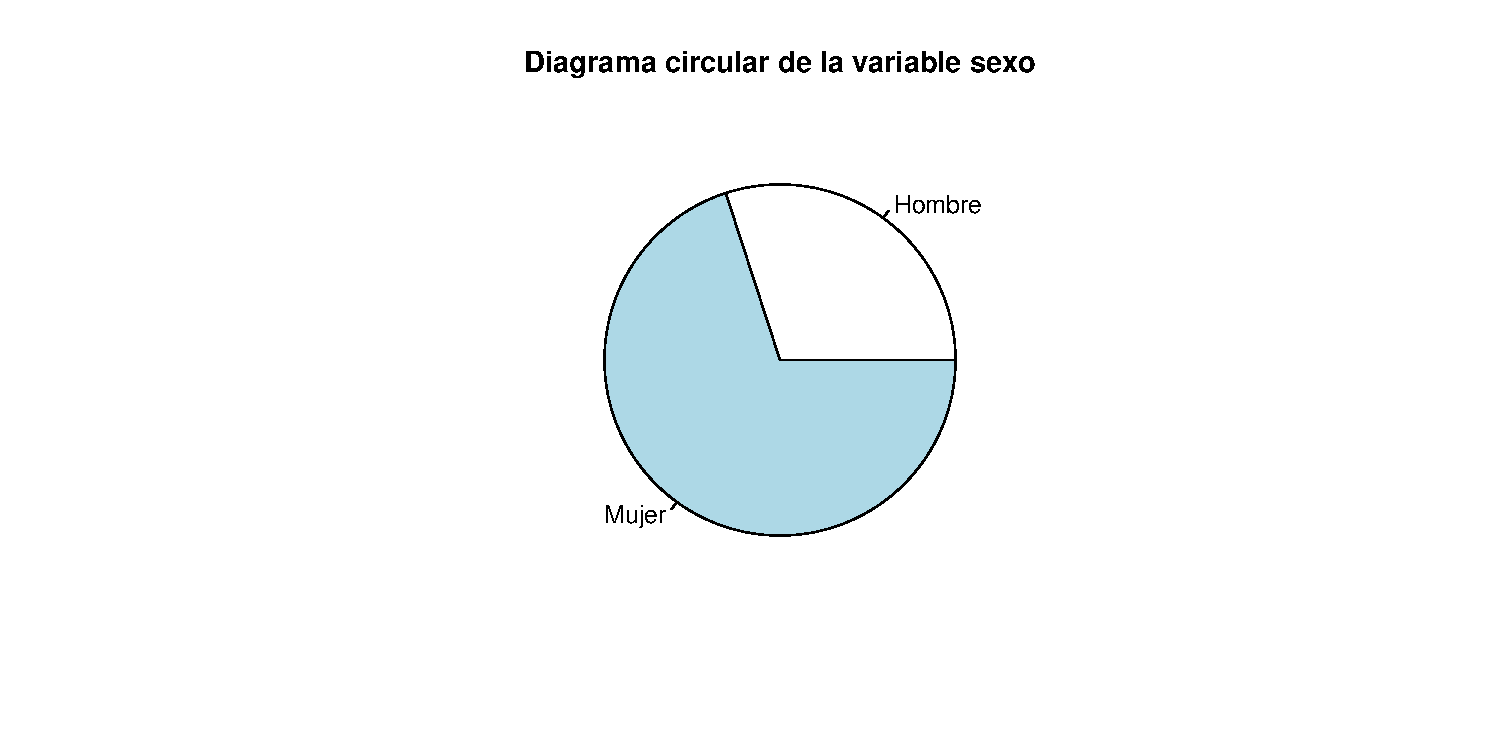
\includegraphics{./dibujos/01/-001}
\end{center}
\end{frame}

\begin{frame}
\frametitle{Ejemplo: gráficos}
\begin{center}
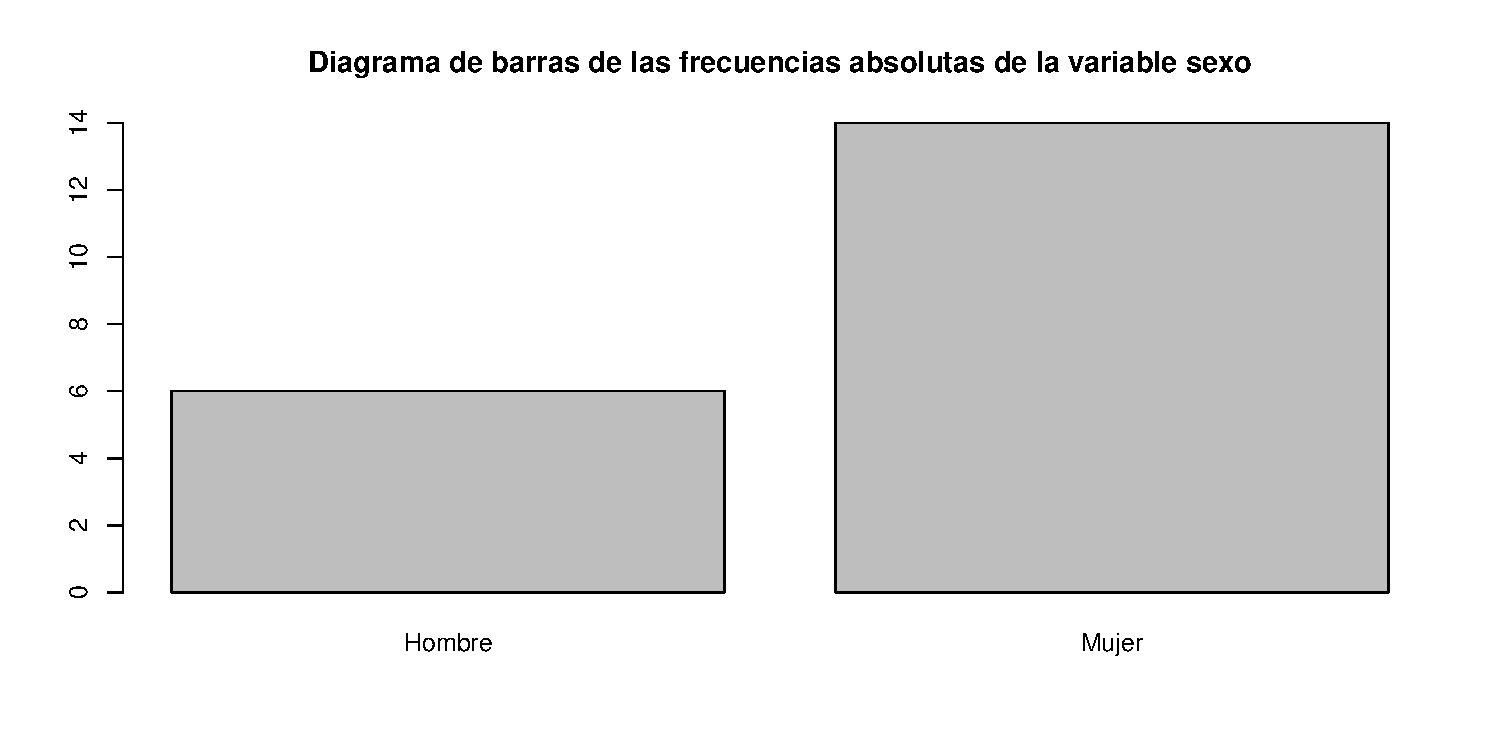
\includegraphics{./dibujos/01/-002}
\end{center}
\end{frame}

\begin{frame}
\frametitle{Ejemplo: gráficos}
\begin{center}
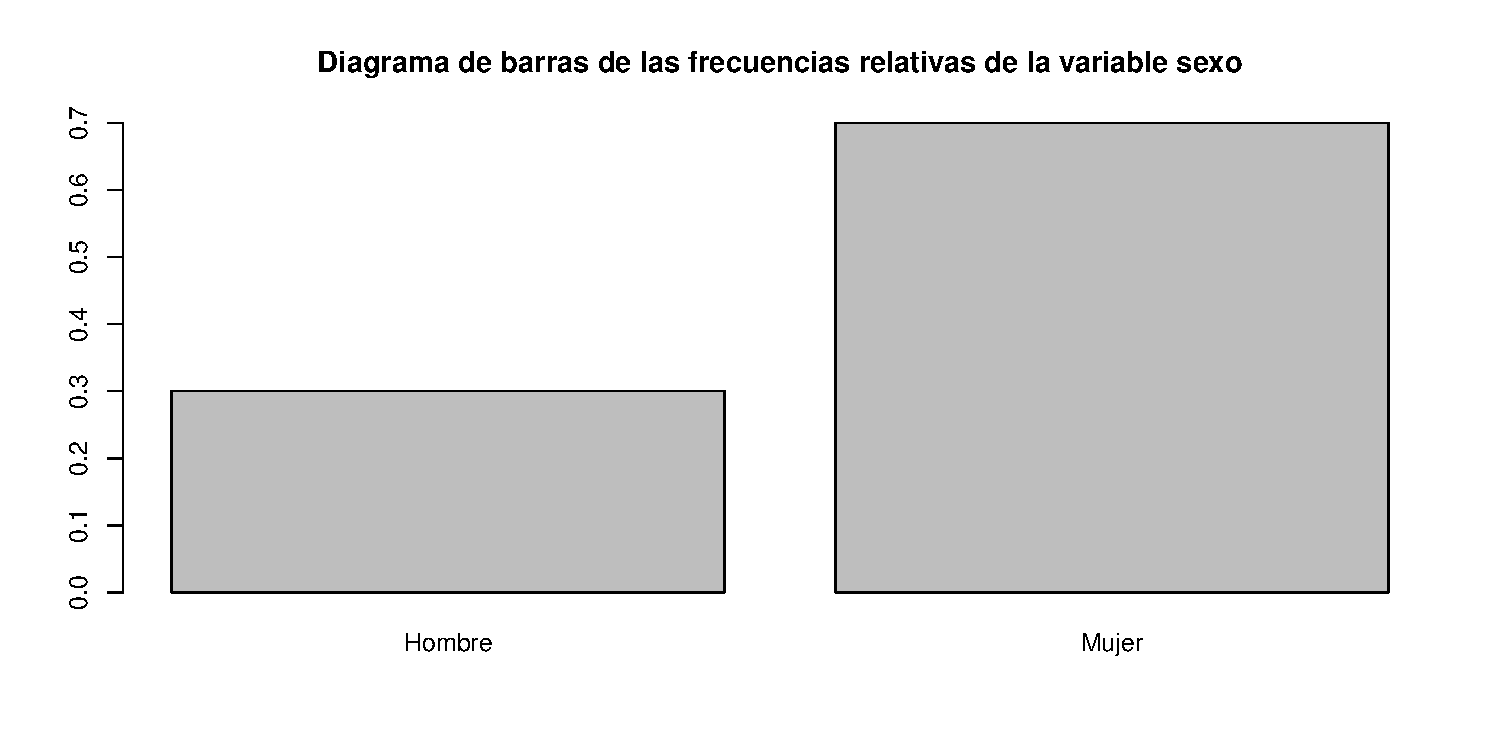
\includegraphics{./dibujos/01/-003}
\end{center}
\end{frame}

\subsection{Datos ordinales}
\begin{frame}
\frametitle{Datos ordinales}
\begin{itemize}
\item Los datos ordinales son variables de tipo cualitativo pero que tienen un orden.
\item  La escala \textsl{Likert} que se utiliza para saber la opinión de un grupo de personas sobre un tema determinado aporta datos
ordinales.
\item Por ejemplo, para saber  el comportamiento \textbf{ético} de la empresa para la que trabajaban un grupo  técnicos de impacto ambiental se les hizo la pregunta siguiente: ¿Cree usted que los técnicos de  impacto ambiental son animados por sus empresas para que  utilicen métodos que favorezcan la opinión del cliente que ha encargado el estudio?
\end{itemize}
\end{frame}

\begin{frame}
\frametitle{Ejemplo: ética}
Las posibles respuesta son una escala ordinal del tipo \textsl{Likert}:
\begin{table}[h]
\begin{center}
\caption{Un ejemplo de datos ordinales}
\begin{tabular}{|r|l|}
\hline
 Nivel  & Significado\\\hline
1 & Bastante en desacuerdo\\
2 & Algo en desacuerdo \\
3 & neutral\\
4 & Algo de acuerdo\\
5 & Bastante de acuerdo\\\hline
\end{tabular}
\end{center}
\end{table}
\end{frame}

\begin{frame}
\frametitle{Notaciones básicas para variables ordinales}


\begin{itemize}
\item Consideremos una variable ordinal que toma los valores $l_1< l_2<\cdots < l_k$.
\item Consideremos las observaciones de estos niveles sobre $n$ individuos \break $x_1,x_2,\ldots,x_n$.
 \item  Las definiciones de \textbf{frecuencias absolutas} ($n_j$), \textbf{frecuencias relativas} ($f_j$) y \textbf{moda} son las misma que para datos cualitativos.
\item La diferencia es que podemos definir la \textbf{frecuencia absoluta acumulada} del valor $l_j$ como $N_j=\sum_{i=1}^j n_i$. Es decir $N_j$ es el número observaciones tales que $x_i< l_j$.
\end{itemize}
\end{frame}

\begin{frame}
\frametitle{Estadísticos básicos variables ordinales}
\begin{itemize}

\item La \textbf{frecuencia relativas acumulada} del valor $l_j$ se definen como $F_j=\frac{N_j}{n}=\sum_{i=1}^j f_i$
\item Notemos que $N_k=n$, $\sum_{j=1}^k f_j=1$ y $F_k=1$.
\item Si queremos obtener porcentajes basta multiplicar por 100 las frecuencias relativas o relativas acumuladas.
\end{itemize}
\end{frame}

\begin{frame}[fragile]
\frametitle{Ejemplo: ética (continuación)}
Supongamos que hemos recogido las respuestas de 100 ($n=100$) técnicos que elaboran informes de impacto ambiental.

Los resultados fueron:
\begin{verbatim}
4 4 2 1 3 3 4 1 1 3 5 2 5 2 1 2 3 2 1 1 2 2 4 2 1
1 1 2 4 5 3 4 2 4 4 3 1 3 3 2 1 5 4 1 2 2 3 3 3 1 
4 3 5 1 5 1 2 5 5 2 4 5 1 4 3 1 1 4 3 3 4 4 1 2 1 
3 4 1 4 2 2 4 1 3 5 3 3 3 2 2 3 3 3 2 4 1 1 4 3 2
\end{verbatim}
\end{frame} 

\begin{frame}
\frametitle{Ejemplo: ética (continuación)}

Construyamos ahora una tabla resumen con todas las frecuencias. En primer primer lugar calculamos las frecuencias absolutas ($n_i$) de cada nivel y a partir de esta el resto de las frecuencias. Notad que en este caso se pueden calcular las frecuencias acumuladas.

% latex table generated in R 2.9.2 by xtable 1.5-6 package
% Fri Jan 22 14:37:48 2010
\begin{table}[ht]
\begin{center}
\begin{tabular}{rrrrr}
  \hline
Valor & $n_i$ & $N_i$ & $f_i$ & $F_i$ \\ 
  \hline
1 &  24 &  24 & 0.24 & 0.24 \\ 
  2 &  22 &  46 & 0.22 & 0.46 \\ 
  3 &  24 &  70 & 0.24 & 0.70 \\ 
  4 &  20 &  90 & 0.20 & 0.90 \\ 
  5 &  10 & 100 & 0.10 & 1.00 \\ 
   \hline
Total & 100 & & 1 & \\\hline
\end{tabular}
\end{center}
\caption{Tabla de frecuencia de los datos ordinales}
\end{table}
 
\end{frame}

\begin{frame}
\frametitle{Gráficos básicos para variables ordinales}

\begin{itemize}
\item Como ya hemos dicho, los gráficos para frecuencias absolutas y relativas son los mismos que para variables cualitativas.
\item Podemos dibujar también los gráficos de frecuencias acumuladas.
\item En principio los diagramas circulares no son adecuados para frecuencias acumuladas.
\end{itemize}


\end{frame}

\begin{frame}
\frametitle{Gráficos básicos para variables ordinales}

\begin{itemize}
\item Los gráficos para frecuencias absolutas y relativas son los mismos que para variables cualitativas.
\item Podemos dibujar también los gráficos de frecuencias acumuladas donde cada barra es proporcional a su frecuencia acumulada y las niveles se colocan, generalmente en orden ascendente. 
\item En principio los diagramas circulares no son adecuados para frecuencias acumuladas.
\end{itemize}


\end{frame}

\begin{frame}
%\frametitle{Ejemplo ética}
\begin{figure}
\begin{center} 
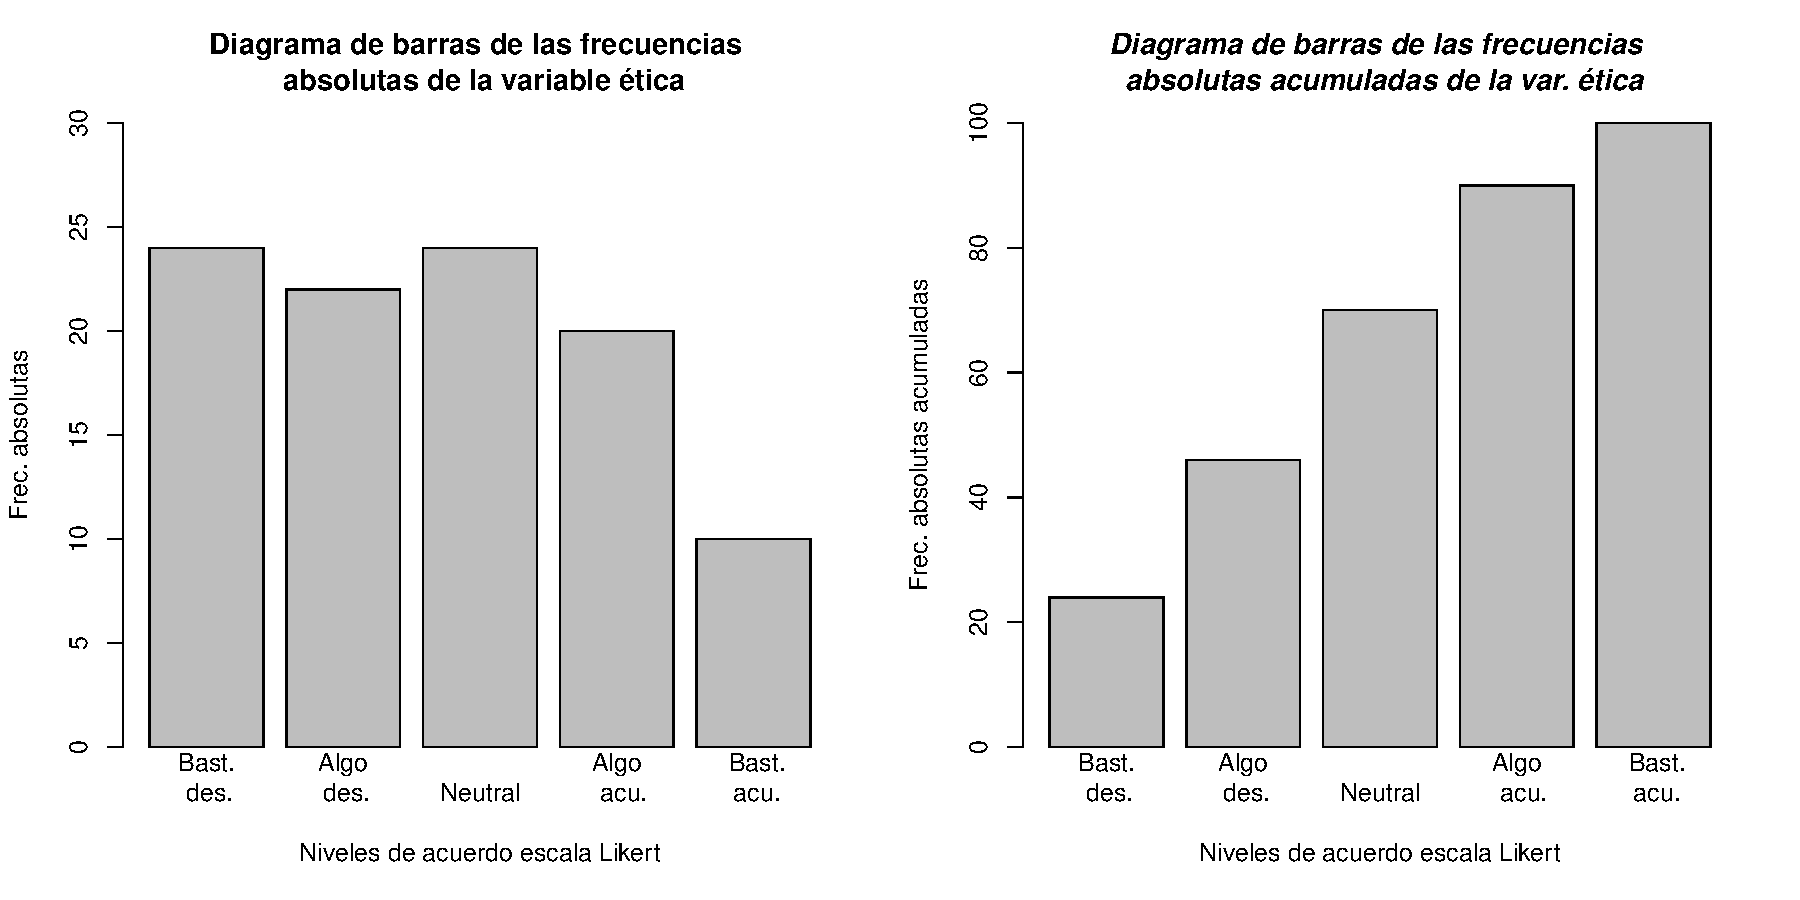
\includegraphics{./dibujos/01/-004}
\caption{Diagrama de barras de datos ordinales frecuencias absolutas y absolutas acumuladas.}
\end{center}
\end{figure} 
\end{frame}


\begin{frame}
%\frametitle{Ejemplo ética}
\begin{figure}
\begin{center} 
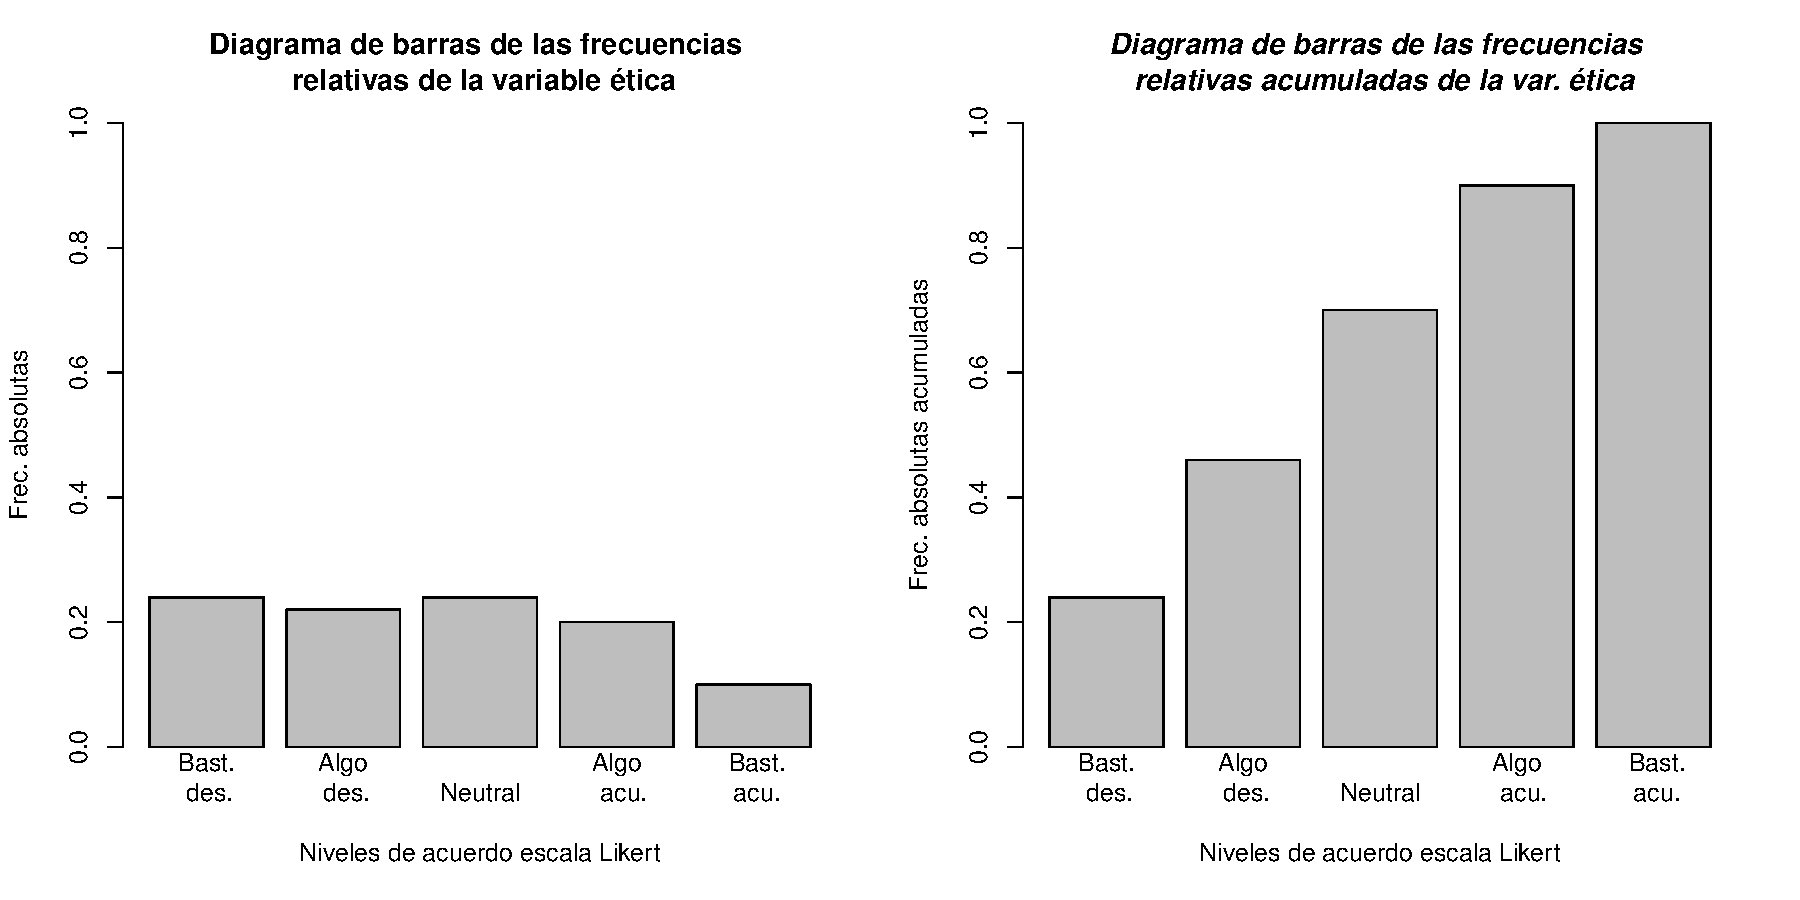
\includegraphics{./dibujos/01/-005}
\caption{Diagrama de barras de datos ordinales frecuencias relativas y relativas acumuladas.}
\end{center}
\end{figure} 
\end{frame}

% \begin{frame}
% \frametitle{Ejemplo ética}
% \begin{figure}
% \begin{center} 
% <<fig =TRUE , echo =FALSE, width=12, height=6 >>=
% etica <- c(4,4,2,1,3,3,4,1,1,3,5,2,5,2,1,2,3,2,1,1,2,2,4,2,1,1,1,2,4,5,3,4,2,4,4,3,1,
% 3,3,2,1,5,4,1,2,2,3,3,3,1,4,3,5,1,5,1,2,5,5,2,4,5,1,4,3,1,1,4,3,3,4,4,1,2,
% 1,3,4,1,4,2,2,4,1,3,5,3,3,3,2,2,3,3,3,2,4,1,1,4,3,2)
% nivelescortodos <- c("Bast.\n des.", "Algo\n des." , "Neutral","Algo\n  acu."," Bast.\n acu.")
% opar <- par(mfrow = c(1,2 ))
% barplot(table(etica),width=0.1,main="Diagrama de barras de las frecuencias \n relativas de la variable ética",font.main = 2,
% names.arg=nivelescortodos,ylim=c(0,1),horiz=F,xlab="Niveles de acuerdo escala Likert",ylab="Frec. absolutas")
% barplot(cumsum(table(etica))/100,main="Diagrama de barras de las frecuencias \n relativas acumuladas de la var. ética",font.main = 4,
% names.arg=nivelescortodos,ylim=c(0,1),horiz=F,xlab="Niveles de acuerdo escala Likert",ylab="Frec. absolutas acumuladas")
% par(opar)
% @
% \caption{Diagrama de barras de datos ordinales frecuencias relativas y relativas acumuladas.}
% \end{center}
% \end{figure} 
% \end{frame}


\subsection{Datos cuantitativos}

\begin{frame}
\frametitle{Datos cuantitativos}
\begin{itemize}
\item  Los datos cuantitativos son los que expresan cantidades que se representan por números.
\item  Por ejemplo los datos que cuentan cosas o que miden pesos, distancias, tiempos, concentraciones....
\item  Entre otras clasificaciones, los datos cuantitativos pueden ser \textbf{discretos} o \textbf{continuos} ....
\end{itemize}
\end{frame}

\begin{frame}
\frametitle{Datos cuantitativos}
\begin{itemize}
\item  Los datos continuos son los que toman valores en intervalos de la recta real.
\item  Los datos  discretos son los que toman un número finito  o infinito, pero contable, de valores.
\item  Por ejemplo los resultados de lanzar un dado de parchís 10 veces y anotar el número de puntos observado 
 son datos discretos.
\item  También lo son el número de nuevas crías de una manada, el número de aminoácidos de una proteína, \ldots
\item  Son datos continuos la edad, el peso, la estatura de un individuo, \ldots 
\end{itemize}

\end{frame}

\begin{frame}
\frametitle{Notación datos cuantitativos}
La notación se diferencia de la de los datos cualitativos y ordinales en que no tenemos porqué disponer de todos los ``niveles''.
\begin{itemize}
\item Sean  $x_1,\ldots,x_n$ las observaciones  cuantitativas sobre un conjunto de $n$ individuos.
\item Denotemos por  $X_1,\ldots,X_k$  a los distintos valores que aparecen en las observaciones.
\item Al ser los datos  numéricos tienen orden y  los etiquetaremos de menor a mayor, así que 
$$X_1 < X_2 < \ldots < X_k.$$
\end{itemize}
\end{frame}

\begin{frame}
\frametitle{Principales estadísticos datos cuantitativos}
\begin{itemize}
\item Llamaremos frecuencia absoluta de $X_j$  y la denotaremos con $n_j$ al número de datos de la muestra que son iguales a $X_j$.
\item Llamaremos frecuencia absoluta acumulada de $X_j$  y la denotaremos con $N_j$ al número de datos de la muestra que son menores o iguales a $X_j$. Obviamente $N_j=\sum_{i=1}^j n_i$.
\item Llamaremos $N_j$ a la frecuencia absoluta acumulada del valor $X_j$ al número de valores $x_i$ tales que  $x_i\leq X_j$.
\item Llamaremos frecuencia relativa  del valor $X_j$ a $f_j=\frac{n_i}{n}$.
\item Llamaremos frecuencia relativa acumulada del valor $X_j$ a $F_j=\sum_{i=1}^j f_i=\frac{N_j}{n}$.
\end{itemize}
\end{frame}


\begin{frame}
\frametitle{Propiedades}

La siguientes propiedades se deducen de forma sencilla:

\begin{itemize}
\item $n_j=N_j-N_{j-1}$, $f_j=F_j-F_{j-1}$.
\item $\sum_{j=1}^k n_j=n$, $\sum_{i=1}^k f_i=1$.
\item $N_k=n$, $F_k=1$, 
\end{itemize}
\end{frame}

\begin{frame}[fragile]
\frametitle{Ejemplo}

\begin{itemize}
\item Lanzamos un dado de parchís  diez veces  $n=10$
\item Los resultados son $x_1=1,x_2=2,x_3=1,x_4=4,x_5=5,x_6=6,x_7=3,x_8=5,x_9=6,x_{10}=3$
\item Los tipos de valores observados son $X_1=1,X_2=2,X_3=3,X_4=4,X_5=5,X_6=6$
\item Podemos resumir todas las frecuencias en  forma de tabla:
\end{itemize}
% latex table generated in R 2.9.2 by xtable 1.5-6 package
% Sun Jan 24 13:21:57 2010
\begin{table}[ht]
\begin{center}
\begin{tabular}{rrrrr}
  \hline
 $X_j$ & $n_j$ & $N_j$ & $f_j$ & $F_j$ \\ 
  \hline
1 &   2 &   2 & 0.20 & 0.20 \\ 
  2 &   1 &   3 & 0.10 & 0.30 \\ 
  3 &   2 &   5 & 0.20 & 0.50 \\ 
  4 &   1 &   6 & 0.10 & 0.60 \\ 
  5 &   2 &   8 & 0.20 & 0.80 \\ 
  6 &   2 &  10 & 0.20 & 1.00 \\ 
   \hline
\end{tabular}
\end{center}
\end{table}
\end{frame}





\begin{frame}
\frametitle{Presentación  frecuencia datos cuantitativos}
Una tabla genérica para representar las frecuencias es la que sigue:
$$
\begin{tabular}{|c|c|c|c|c|}
\hline $X_j$ & $n_j$ & $N_j$ & $f_j$ & $F_j$ \\ \hline \hline $X_1$ & $n_1$ & $N_1$ &
$f_1$ & $F_1$ \\ \hline $X_2$ & $n_2$ & $N_2$ & $f_2$ & $F_2$ \\ \hline $\vdots$ &
$\vdots$ & $\vdots$ & $\vdots$ & $\vdots$ \\ \hline $X_k$ & $n_k$ & $N_k=n$ & $f_k$ &
$F_k=1$
\\ \hline \hline Total $\sum$ & n & & 1 & \\ \hline
\end{tabular}
$$
\end{frame}


\begin{frame}
\frametitle{Medidas de tendencia central para datos cuantitativos}
Las medidas de tendencia central o estadísticos de tendencia central son las que nos dan un valor representativo de todas las observaciones:
\begin{itemize}
\item \textbf{Moda}: es el valor (o valores) de máxima frecuencia.
\item \textbf{Media aritmética}: $\overline{x}=\frac{\sum_{i=1}^n x_i}{n}=\frac{\sum_{j=1}^k n_j\cdot X_j}{n}=
\sum_{i=j}^k f_j\cdot X_j$.
\item  En lo que sigue cuando hablemos de ``\textsl{la media de unos datos}''  nos referiremos  a la media aritmética salvo que indiquemos lo contrario.
\item Hay otros tipos de medias como: la  \textbf{media aritmética recortada}, la \textbf{ media geométrica} y  la \textbf{media armónica}.
\item Al final de estas notas de estadística descriptiva daremos las fórmulas de estas medias.
\end{itemize}
\end{frame}

\begin{frame}
%\frametitle{Principales estadísticos para datos cuantitativos}
\begin{itemize}
\item \textbf{Los cuantiles}. Dado un valor $0<p<1$ llamaremos cuantil de orden $p$ y lo denotaremos por $Q_p$ al valor mas pequeño cuya frecuencia relativa acumulada es mayor o igual a $p$.
\item \textbf{La mediana, los cuartiles, los deciles, los percentiles}
\begin{itemize}
\item \textbf{La mediana} es el valor más pequeño que deja su izquierda al menos la mitad de los datos, es decir es $Q_{0.5}$.
\item \textbf{Los cuartiles}: son los cuantiles $Q_{0.25},Q_{0.5},Q_{0.75}$ que reciben el nombre de primer cuartil, segundo cuartil (o mediana) y tercer cuartil respectivamente. Son los valores más pequeños que dejan a su izquierda al menos la cuarta parte de los datos, la mitad de los datos y las tres cuartas partes de los datos.
\item No existe un consenso para el cómputo  de estos valores. En \texttt{R} la función \texttt{quantile} tiene hasta $9$ maneras de calcular estos valores.
\end{itemize}
\end{itemize}
\end{frame}


\begin{frame}
%\frametitle{Principales estadísticos para datos cuantitativos}
\frametitle{El cálculo de la mediana}
\begin{itemize}
\item En este caso sí hay un consenso general para su cálculo.
\item Supongamos que tenemos una muestra de datos: $x_1,x_2,\ldots, x_n$.
\item Denotaremos por $x_{(1)}\leq x_{(2)}\leq \cdots \leq x_{(n)}$ la muestra ordenada de menor a mayor.
\item Calcularemos la mediana, $Q_{0.5}$, de la siguiente forma:

$$Q_{0.5}=\left\{\begin{array}{ll}
\frac{x_{\left(\frac{n}{2}\right)}+x_{\left(\frac{n}{2}+1\right)}}{2} & \mbox{ si } n \mbox{ es par}\\
x_{\left(\frac{n+1}{2}\right)} & \mbox{ si  }  n \mbox{ es impar}\end{array}\right.
$$
\end{itemize}
\end{frame}





\begin{frame}
%\frametitle{Principales estadísticos para datos cuantitativos}
\frametitle{El cálculo de la mediana}

En este caso sí hay un consenso general para su cálculo. Supongamos que tenemos una muestra de datos: $x_1,x_2,\ldots, x_n$

Denotaremos por $x_{(1)}\leq x_{(2)}\leq \cdots \leq x_{(n)}$ la muestra ordenada de menor a mayor.

Calcularemos la mediana, $Q_{0.5}$, de la siguiente forma:

$$Q_{0.5}=\left\{\begin{array}{ll}
\frac{x_{\left(\frac{n}{2}\right)}+x_{\left(\frac{n}{2}+1\right)}}{2} & \mbox{ si } n \mbox{ es par}\\
x_{\left(\frac{n+1}{2}\right)} & \mbox{ si  }  n \mbox{ es impar}\end{array}\right.
$$
\end{frame}


\begin{frame}
%\frametitle{Principales estadísticos para datos cuantitativos}
\frametitle{El cálculo de los cuartiles}
\begin{itemize}
\item En este caso no hay un consenso general para su cálculo.
\item La instrucción \texttt{R quantile} dispone de hasta $9$ maneras de cálculo.
\item Supongamos que tenemos una muestra de datos: $x_1,x_2,\ldots, x_n$.
\item Denotaremos por $x_{(1)}\leq x_{(2)}\leq \cdots \leq x_{(n)}$ la muestra ordenada de menor a mayor.
\item Calcularemos el primer cuartil, $Q_{0.25}$, de la siguiente forma:

$$Q_{0.25}=\left\{\begin{array}{ll}
\mbox{la mediana de } x_{(1)},x_{(2)},\ldots,x_{(\frac{n}{2})} & \mbox{ si } n \mbox{ es par}\\
\mbox{la mediana de } x_{(1)},x_{(2)},\ldots,x_{(\frac{n+1}{2})} & \mbox{ si } n \mbox{ es impar}\\
\end{array}\right.
$$

\item Mientras que para el tercer cuartil:
$$Q_{0.75}=\left\{\begin{array}{ll}
\mbox{la mediana de } x_{(\frac{n}{2})},x_{(\frac{n}{2}+1)},\ldots,x_{n} & \mbox{ si } n \mbox{ es par}\\
\mbox{la mediana de } x_{(\frac{n+1}{2})},x_{(\frac{n+1}{2}+1)},\ldots,x_{(n)} & \mbox{ si } n \mbox{ es impar}\\
\end{array}\right.
$$
\end{itemize}
\end{frame}


\begin{frame}
\frametitle{Ejemplo}

Consideremos el siguiente conjunto de datos:

$$x_1=6 x_2=3, x_3=2, x_4= 1 x_4=5,x_6=6.$$

El número de datos es $n=6$ y su media aritmética es 

$$\overline{x}=\frac{\sum_{i=1}^n x_i}{n}=\frac{6+3+2+1+5+6}{6}=\frac{23}{6}=3.8333.$$

\end{frame}

\begin{frame}
\frametitle{Ejemplo}

 La tabla de frecuencias de estos datos es:


% latex table generated in R 2.9.2 by xtable 1.5-6 package
% Mon Jan 25 18:55:43 2010
\begin{table}[ht]
\begin{center}
\begin{tabular}{rrrrr}
  \hline
$X_j$ & $n_j$ & $N_j$ & $f_j$ & $F_j$ \\ 
  \hline
  1 & 1 & 1 & 0.1667 & 0.1667 \\ 
  2 & 1 & 2 & 0.1667 & 0.3333 \\ 
  3 & 1 & 3 & 0.1667 & 0.5000 \\ 
  5 & 1 & 4 & 0.1667 & 0.6667 \\ 
  6 & 2 & 6 & 0.3333 & 1.0000 \\ 
   \hline
Total & $n=6$ & & 1 & \\\hline
\end{tabular}
\end{center}
\end{table}

Todos los cálculos se han redondeado hasta el cuarto decimal.
\end{frame}





\begin{frame}
%\frametitle{Ejemplo sencillo}
Para los cálculos de la media con frecuencias se suele ampliar esta tabla como sigue:
% latex table generated in R 2.9.2 by xtable 1.5-6 package
% Mon Jan 25 18:52:44 2010
\begin{table}[ht]
\begin{center}
\begin{tabular}{rrrrrrr}
  \hline
$X_j$ & $n_j$ & $N_j$ & $f_j$ & $F_j$ & $n_j\cdot X_j$ & $f_j\cdot X_j$ \\ 
  \hline
1 & 1 & 1 & 0.1667 & 0.1667 & 1.0000 & 0.1667 \\ 
  2 & 1 & 2 & 0.1667 & 0.3333 & 2.0000 & 0.3333 \\ 
  3 & 1 & 3 & 0.1667 & 0.5000 & 3.0000 & 0.5000 \\ 
  5 & 1 & 4 & 0.1667 & 0.6667 & 5.0000 & 0.8333 \\ 
  6 & 2 & 6 & 0.3333 & 1.0000 & 12.0000 & 2.0000 \\ 
   \hline
Total & $n=6$  &  & 1 & & 23 & 3.8333\\
\end{tabular}
\end{center}
\end{table}

Así, con los datos obtenidos de los totales de las columnas, tenemos que  $\overline{x}=\frac{23}{6}=3.8333$.
\end{frame}

\begin{frame}
%\frametitle{Ejemplo}

Calculemos ahora la mediana. Los datos ordenados de menor a mayor son:


$$x_{(1)}=1, x_{(2)}=2, x_{(3)}=3 x_{(4)}= 5, x_{(5)}=6, x_{(6)}=6.$$


Como $n=6$ es par  tenemos que:

$Q_{0.5}=\frac{x_{\left(\frac{n}{2}\right)}+x_{\left(\frac{n}{2}+1\right)}}{2} =\frac{x_{\left(\frac{6}{2}\right)}+x_{\left(\frac{6}{2}+1\right)}}{2} =
\frac{x_{(3)}+x_{(4)}}{2} =\frac{3+5}{2}=4.$
\end{frame}

\begin{frame}
\frametitle{Medidas de dispersión  para datos cuantitativos}
Las medidas de dispersión o estadísticos de dispersión, son los que nos dan un valor de los alejados que están entre sí los datos:
\begin{itemize}
\item \textbf{Rango}: Es la diferencia entre el máximo y el mínimo de las observaciones.
\item \textbf{Rango intercuartílico}: Es la diferencia entre el tercer cuartil y el primer cuartil $Q_{0.75}-Q_{0.25}$.
\end{itemize}
\end{frame}

\begin{frame}
%\frametitle{Principales estadísticos para datos cuantitativos}
%\textbf{Medidas de dispersión, continuación:}
\begin{itemize}
\item La \textbf{desviación cuadrática del dato} $x_i$ respecto de la media es $(x_i-\overline{x})^2$.
\item \textbf{La varianza}:  La media de las desviaciones cuadráticas respecto de la media es la varianza.
\item \textbf{Fórmulas de la varianza}:
 $s^2=\frac{\sum_{i=1}^n (x_i-\overline{x})^2}{n}=\frac{\sum_{i=1}^n n_i\cdot (X_i-\overline{x})^2}{n}=\sum_{i=1}^n f_i\cdot (X_i-\overline{x})^2.$
\item \textbf{La desviación típica}: Es la raíz cuadrada positiva de la varianza $s=+\sqrt{s^2}$.

\end{itemize}
\end{frame}

\begin{frame}
\frametitle{Principales estadísticos para datos cuantitativos}
\textbf{Medidas de dispersión, continuación:}
\begin{itemize}
\item \textbf{La cuasivarianza}: Es una corrección de la varianza la denotamos y se calcula  con  $\tilde{s}^2 =
\frac{n-1}{n} \cdot s^2.$
\item \textbf{Fórmulas de la cuasi varianza}:
 $$s^2=\frac{\sum_{i=1}^n (x_i-\overline{x})^2}{n-1}=\frac{\sum_{i=1}^n n_i\cdot (X_i-\overline{x})^2}{n-1}-$$
\item \textbf{La cuasi desviación típica}: Es la raíz cuadrada positiva de la cuasi varianza $\tilde{s}=+\sqrt{\tilde{s}^2}$.
\item Hay otras medidas de dispersión como la desviación media o la desviación respecto de la mediana ...
\end{itemize}
\end{frame}


\begin{frame}
\frametitle{Algunas propiedades de la varianza}

\begin{itemize}
\item La varianza siempre es mayor o igual que cero: $s^2\geq 0$.
\item Si $s^2=0$ entonces todos los datos son iguales. Dicho de otro modo los datos son constantes y por lo tanto
 iguales a su media.
\item De todas las desviaciones medias  cuadráticas respecto  de un punto, la varianza es la más pequeña. Más formalmente:

$$s^ 2 \leq \frac{\sum_{i=1}^n (x_i- M)^ 2}{n}$$


para cualquier valor $M$.

% \item  La propiedad anterior significa que la varianza puede  utilizarse para comparar variabilidades de distintos conjuntos de datos.
\end{itemize}
\end{frame}

\begin{frame}
\frametitle{Algunas propiedades de la varianza}

\begin{itemize}
\item $s^2= \frac{\sum_{i=1}^n x_i^2}{n}-\overline{x}^2=\frac{\sum_{j=1}^k n_j\cdot X_j^2}{n}-\overline{x}^2=\sum_{j=1}^k f_j \cdot X_j^2-\overline{x}^2.$
\item $\tilde{s}^2=\frac{\sum_{i=1}^n x_i^2}{n-1}-\frac{n}{n-1}\cdot \left(\overline{x}^2 \right)=\frac{\sum_{i=1}^n x_i^2- \frac{1}{n}\cdot \left(\sum_{i=1}^n x_i\right)^2}{n-1}.$
\item $\tilde{s}^2=\frac{\sum_{j=1}^k n_j\cdot  X_j^2}{n-1}-\frac{n}{n-1}\cdot \left(\overline{x}^2 \right)=\frac{\sum_{j=1}^k
n_j\cdot X_j^2- \frac{1}{n} \cdot \left(\sum_{i=1}^k n_j\cdot X_j\right)^2}{n-1}.$
%\item $\tilde{s}^2=\sum_{j=1}^k f_j\cdot X_j^2- \frac{1}{n} \cdot \left(\sum_{i=1}^k f_j\cdot X_j\right)^2.$
\end{itemize}
\end{frame}

\begin{frame}
\frametitle{Ejemplo}
\begin{itemize}
\item Sigamos con los datos del ejemplo anterior:

$$x_1=6 x_2=3, x_3=2, x_4= 1 x_4=5,x_6=6.$$

\item El número de datos es $n=6$ y su media aritmética es $$\overline{x}=3.8333.$$

\item Queremos calcular la varianza, la desviación típica, la cuasivarianza y la cuasi desviación típica. Cuando sea necesario redondearemos hasta el cuarto decimal.
\end{itemize}
\end{frame}

\begin{frame}
\frametitle{Ejemplo}
Reconstruyamos parte de la tabla de frecuencia y la ampliaremos para nuestros cálculos:
% latex table generated in R 2.9.2 by xtable 1.5-6 package
% Wed Jan 27 19:59:45 2010
\begin{table}[ht]
\begin{center}
\begin{tabular}{rrrrr}
  \hline
$X_j$ & $n_j$ & $n_j\cdot X_j$ & $n_j\cdot \left(X_j-\overline{x}\right)^2$ & $n_j\cdot X_j^2$ \\ 
  \hline
1 & 1 & 1 & 8.0276 & 1 \\ 
  2 & 1 & 2 & 3.3610 & 4 \\ 
  3 & 1 & 3 & 0.6944 & 9 \\ 
  5 & 1 & 5 & 1.3612 & 25 \\ 
  6 & 2 & 12 & 9.3892 & 72 \\ 
   \hline
Total &  6 &  23 &  22.8333 &  111
\end{tabular}
\end{center}
\end{table}
En la última fila de tabla   obtenemos los totales de las columnas.
\end{frame}

\begin{frame}
%\frametitle{Ejemplo sencillo}
Por lo tanto (redondeando siempre al cuarto decimal):
\begin{itemize}
 \item  Como $\sum_{j=1}^5 n_j=n=6,\quad \sum_{j=1}^5 n_j\cdot x_j=23$ tenemos que $ \overline{x}=\frac{23}{6}=3.8333$
\item Como $\sum_{j=1}^5 ni\cdot(X_j-\overline{x})^2=22.8333$ tenemos que $s^2=\frac{22.8333}{6}=3.8056$ y que $\tilde{s}^2=\frac{22.8333}{5}=4.5667$.
\item Como $\sum_{j=1}^5 ni\cdot X_j^2=111$ tenemos que $s^2=\frac{111}{6}-3.833^2= 3.8058$ 
y $\tilde{s}^2=\frac{111}{5}-\frac{6}{5} 3.833^2= 4.5697$.
\item  Las discrepacias son debidas al redondeo.
\item Se deja como ejercicio calcular la desviación típica y la cuasi desviación típica y también repetir estos cálculos con las fórmulas de las frecuencias relativas.
\end{itemize}
\end{frame}

\section{Datos agrupados}
\begin{frame}
 \frametitle{Agrupamiento de datos}
\begin{itemize}
\item Los datos discretos son más fáciles de observar. Cuando un dato responde a un conteo  suele ser fácil estimar de forma exacta el resultado. En otras ocasiones  es más difícil como por  ejemplo:
\begin{itemize}
\item Cuando los datos son continuos y de una precisión elevada, como por ejemplo el peso, el tiempo
\item O en ocasiones, discretos con un número elevado de posibles valores
 (número de aminoácidos de una proteína).
\end{itemize}
\item Se corre el riesgo de que las frecuencias resuman escasamente la muestra, es decir que las
frecuencias absolutas de cada valor sean $1$ o  a lo más $2$.
\item Este conteo de frecuencias es poco útil para estudiar el comportamiento de los datos.
\item  En ambos casos se suele recurrir al conteo de datos por grupos o intervalos de valores a los que se denomina
clases; es lo que se llama recuento de datos agrupados.
\end{itemize}
\end{frame}
\begin{frame}

\frametitle{Los intervalos}
\begin{itemize}
\item Consideremos el caso del peso en kilogramos de una persona. Cuando decimos yo peso 60
kilos ¿qué estoy diciendo en realidad? 
\item Si consideramos la edad y digo que tengo 21 años
¿qué estoy diciendo en realidad?
\item En la variable continua ``peso en kilos'' tenemos que los
valores se calculan hasta las unidades
\item  Si estamos tomando una medida en forma correcta
decir que pesamos 60 Kg. debería ser equivalente a decir que pesamos $60\pm 0.5$ Kg
%\item Es decir nuestro instrumento de medida debería medir así.
\end{itemize}
\end{frame}

\begin{frame}
%\frametitle{Los intervalos}
\begin{itemize}
\item El error cometido será la mitad de la precisión del instrumento de medida.
\item  Lo mismo sucede con la edad; cometemos menos error si decimos que tenemos 18 años cuando tengamos $18\pm 0.5$ años.
\item Evidentemente en la vida real no se hace así. Si digo que tengo 19 años queremos decir que nuestra edad está en el intervalo $[19,20)$.
\item  Si utilizamos esta forma de medir, el error de medida es la mitad de la precisión.
\end{itemize}
\end{frame}

\begin{frame}
\frametitle{ ¿En qué consiste agrupar datos?}
Supongamos que disponemos de un conjunto de datos $x_1,x_2,\ldots, x_n$, del que conocemos su precisión.
Queremos agrupar los datos por intervalos para contar las frecuencia por grupos, para ello:
\begin{itemize}
\item Necesitamos decidir el número de intervalos. Estos intervalos reciben el nombre de \textbf{clases}. Denotaremos su número por $k$.
\item El número de intervalos  puede ser determinado por el interesado. También se puede determinar con distintas formas como la de regla de Sturges, la regla de Scott o la regla de Freedman and Diaconis:
\end{itemize}
\end{frame}

\begin{frame}
\begin{itemize}
\item  Regla de Sturges: $k= \lceil 1+\log_{2}(n) \rceil.$
\item  Regla de Scott: Determina primero la amplitud $A$ de las clases  $A= 3.5 \cdot s \cdot n^{-\frac{1}{3}}$ y  ahora $k=\lceil \frac{(\mbox{máx} -\mbox{mín})}{A}\rceil$.
\item  Regla de Freedman and Diaconis: Determina primero la amplitud $A$ de las clases  $A= 2 \cdot (Q_3-Q_2) \cdot n^{-\frac{1}{3}}$ y  ahora $k=\lceil \frac{(\mbox{máx} -\mbox{mín})}{A}\rceil$.
\item La función $\lceil x \rceil$= al menor entero superior a $x$, es la llamada función ``techo'' (\textsl{ceiling}).
\end{itemize}
\end{frame}

\begin{frame}
%\frametitle{ ¿En qué consiste agrupar datos?}
\begin{itemize}
\item Una vez determinado el valor de $k$, necesitamos determinar la amplitud de los intervalos $A_i$. La forma más sencilla es suponer que todos los intervalos son de igual amplitud $A$ y calcular ésta, redondeándola por exceso a un valor de la precisión de la medida.
\item Por ejemplo si la precisión es el 1 Kilo, k=7, y el rango de nuestros datos es 30, como $\frac{30}{7}=4.2857$, el valor de $A=5$.
\item Elegir el extremo inferior y superior del intervalo de cada clase. Los denotaremos por $[L_1,L_2),[L_2,L_3),\ldots, [L_k,L_{k+1})$.
\end{itemize}
\end{frame}

\begin{frame}
\begin{itemize}
\item  El extremo más pequeño $L_1$ se calcula como $L_1=\mbox{mínimo}-\mbox{precisión}/2$, el siguiente será $L_2=L_1+A$, y así sucesivamente $L_j=L_{j-1}+A$.
\item Determinar las marcas de clase de cada intervalo $X_j$. Como regla general se toma como marca el punto medio de cada intervalo $X_j=\frac{L_{j+1}+L_j}{2}$. En ocasiones se  eligen otras marcas de clase para los intervalos de los extremos.
\end{itemize}
\end{frame}

\begin{frame}
\frametitle{ Ejemplo alergia (S. Milton pág 27)}
Mucha gente manifiesta reacciones alérgica sistémica a las picaduras de insectos. Estas reacciones varían de paciente en paciente, no sólo en cuanto a la gravedad, sino también en el tiempo transcurrido hasta que se inicia la reacción. Los datos siguientes representan ese ``tiempo de inicio hasta la reacción'' en 40 pacientes que experimentaron una reacción sistémica a la picadura de abeja. Los datos están en minutos.

10.5 11.2 9.9 15.0 11.4 12.7 16.5 10.1 12.7 11.4 11.6 6.2 7.9 8.3 10.9 8.1 3.8 10.5 11.7 8.4 12.5 11.2 9.1 10.4 9.1 13.4 12.3 5.9 11.4 8.8 7.4 8.6 13.6 14.7 11.5 10.9 9.8 12.9 9.9
\end{frame}

\begin{frame}
%\frametitle{Ejemplo alergia}
\begin{itemize}
\item El este caso la precisión de los datos es la décima de segundo.
\item El número de datos es $n=40$, la regla de Sturges consiste en tomar el entero superior a $1+\log_{2}(n)$. 
En nuestro caso $1+\log_{2}(40)=6.3219$ por lo tanto $k=7$ intervalos
El mínimo y el máximo son $3.8$ y $16.5$ respectivamente. Así el rango es $16.5-38=12.7$.
\item Tomaremos todos los intervalo de de igual amplitud $A$. Como  el rango dividido por $k$ es $12.7/7= 1.8143$.
Redondeando la amplitud a  la precisión por exceso obtenemos que $A=1.9$.
\end{itemize}
\end{frame}

\begin{frame}
%\frametitle{Ejemplo alergia}
\begin{itemize}
\item Así los extremos de las clases serán $L_1=3.8-0.05=3.75$, $L_2=L_1+1.9=5.65$ y sucesivamente
$L_3= 7.55, L_4=  9.45, L_5= 11.35, L_6= 13.25, L_7= 15.15, L_8= 17.05$.
\item Las marcas de clase  son $X_1=4.7, X_2=6.6, X_3= 8.5, X_4=  10.4, X_5= 12.3, X_6= 14.2, X_7= 16.1$.
\end{itemize}
\end{frame}

\begin{frame}
%\frametitle{Ejemplo alergia}
Ahora podemos disponer los datos en forma de tabla y calcular las frecuencias absolutas, y sus acumuladas para cada intervalo:
% latex table generated in R 2.9.2 by xtable 1.5-6 package
% Thu Jan 28 00:00:18 2010
\begin{table}[ht]
\begin{center}
\begin{tabular}{rrrrrrr}
  \hline
$[L_j$, & $L_{j+1})$ & $X_j$ & $n_j$ & $N_j$ & $f_j$ & $F_j$ \\ 
  \hline
3.75 & 5.65 & 4.70 &   1 &   1 & 0.03 & 0.03 \\ 
  5.65 & 7.55 & 6.60 &   3 &   4 & 0.07 & 0.10 \\ 
  7.55 & 9.45 & 8.50 &   8 &  12 & 0.20 & 0.30 \\ 
  9.45 & 11.35 & 10.40 &  11 &  23 & 0.28 & 0.58 \\ 
  11.35 & 13.25 & 12.30 &  12 &  35 & 0.30 & 0.88 \\ 
  13.25 & 15.15 & 14.20 &   4 &  39 & 0.10 & 0.97 \\ 
  15.15 & 17.05 & 16.10 &   1 &  40 & 0.03 & 1.00 \\ 
   \hline
\end{tabular}
\end{center}
\end{table}
\end{frame}

\begin{frame}
\frametitle{Tabla de frecuencias de un conteo agrupado.}
En general en un conteo de datos agrupados las tabla de frecuencias es:
\begin{table}[ht]
\begin{center}
\begin{tabular}{lccccc}
intervalos & \begin{tabular}{c}{\footnotesize (Marca de clase)}\\$X_j$ \end{tabular}  &
$n_j$ & $N_j$ & $f_j$ & $F_j$
\\ \hline \hline $[L_1,L_2)$ & $X_1$ & $n_1$ & $N_1$ & $f_1$ & $F_1$ \\ \hline
$[L_2,L_3)$ & $X_2$ & $n_2$ & $N_2$ & $f_2$ & $F_2$ \\ \hline $\vdots$ & $\vdots$ &
$\vdots$ & $\vdots$ & $\vdots$ & $\vdots$ \\ \hline $[L_k,L_{k+1})$ & $X_k$ & $n_k$ &
$N_k$ & $f_k$ & $F_k$
\\ \hline \hline Suma $\sum$ & & n & & 1 & \\ \hline
\end{tabular}
\end{center}
\end{table}
\end{frame}

\begin{frame}
\frametitle{Ejemplo árboles frutales}

 Consideremos los siguientes datos sobre el número de árboles  afectados por la mosca de la fruta en    $50$ parcelas rústicas.
\begin{center}
\begin{tabular}{cccccccccc}
8 & 11 & 11 & 8 & 9 & 10 & 16 & 6 & 12 & 19 \\ 13 & 6 & 9 & 13 & 15 & 9 & 12 & 16 & 8 & 7
\\ 14 & 11 & 15 & 6 & 14 & 14 & 17 & 11 & 6 & 9 \\ 10 & 19 & 12 & 11 & 12 &  6 & 15 & 16
& 16 & 12 \\ 13 & 12 & 12 & 8 & 17 & 13 & 7 & 12 & 14 & 12
\end{tabular}
\end{center}
\end{frame}

\begin{frame}
\frametitle{Ejemplo árboles frutales}
La tabla de frecuencias agrupadas en  y amplitud fija de los intervalos $A=3$ es:
\begin{table}[h]
\begin{center}
\begin{tabular}{lccccc}
intervalos  & $X_j$ & $n_j$ & $N_j$ &  $f_j$ &  $F_j$ \\ \hline 
$[5.5,8.5)$  & \ 7  & 11
& 11 & 0.22 &  0.22 \\ $[8.5,11.5)$ & 10  & 11  & 22  & 0.22  & 0.44 \\ $[11.5,14.5)$ &
13 & 17  & 39  & 0.34  & 0.78 \\ $[14.5,17.5)$ & 16 & \ 9  & 48 & 0.18  & 0.96 \\
$[17.5,20.5)$ & 19   & \ 2  & 50 & 0.04  & 1.00 \\ \hline
\end{tabular}
\end{center}
\end{table}
\end{frame}

\subsection{Descripción gráfica  datos agrupados}

\begin{frame}
\frametitle{Los histogramas}
\begin{itemize}
\item La descripción gráfica  de los datos agrupados se hace mediante histogramas.
En la fig.~\ref{FAAVQC} tenemos un ejemplo de histograma.
\item En este caso es el histograma
de  las frecuencias absolutas a la izquierda y a la derecha tenemos el gráfico de las
frecuencias absolutas acumuladas.
\end{itemize}
\end{frame}

\begin{frame}
\begin{figure}
\label{FAAVQC}
\begin{center}
%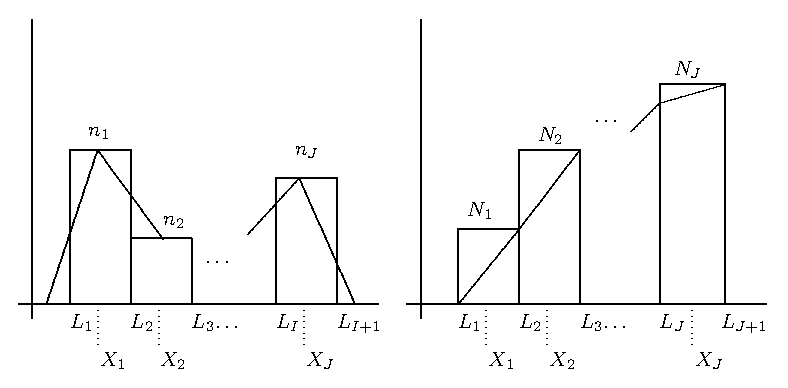
\includegraphics{frecuencias}
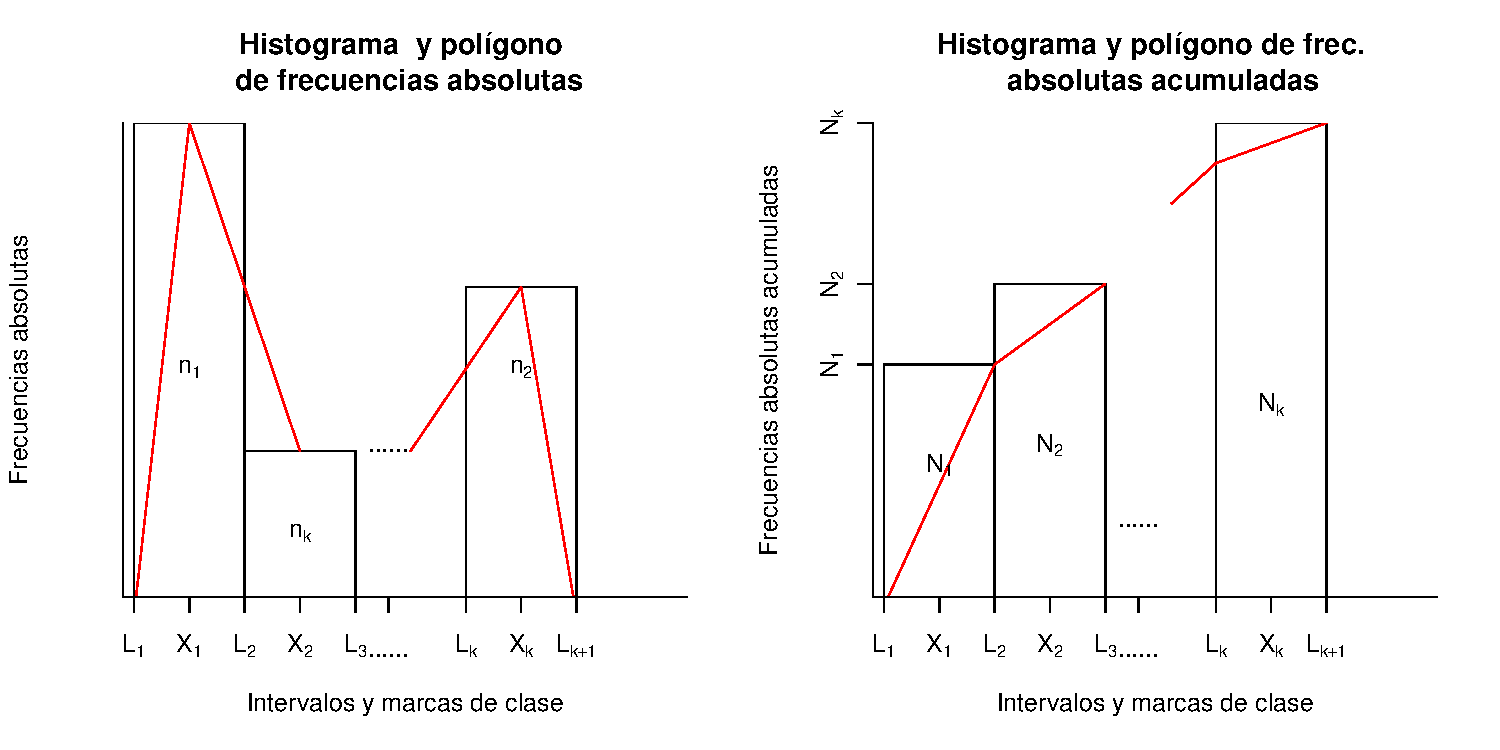
\includegraphics{./dibujos/01/-006}
\end{center}
\caption{Frecuencias absolutas. Variables agrupadas}
\end{figure}
\end{frame}

\begin{frame}
\frametitle{Los histogramas}
\begin{itemize}
\item  Las frecuencias absolutas $n_j$ del gráfico de la
izquierda representen las áreas de los rectángulos de la base $A_j=L_{j+1}-L_j$ la amplitud del
intervalo de clase.
\item  Las frecuencias absolutas acumuladas $N_j$ del gráfico
de la derecha representen las alturas de los rectángulos de base $A_j=L_{i+1}-L_i$.
\item  La curva
 que une los pares ordenados $(X_j,h_j)$ recibe el nombre
  se llama  polígono de frecuencias absolutas (léase igual para relativas).
\item  El polígono de frecuencias absolutas acumuladas (de forma similar para relativas) es el formado por los puntos
  $(L_1,0),(L_2,N_1),\ldots,(L_{k+1},N_k)$.
\end{itemize}
\end{frame}

\begin{frame}
\frametitle{Ejemplo árboles frutales: histograma}
Consideremos los $50$ datos sobre árboles frutales. Tomamos
intervalos  de amplitud $3$. El histograma de frecuencias absolutas con el
correspondientes polígono de frecuencias acumuladas se muestra en la
fig.~\ref{EXEMPLE2}.

Notemos que las alturas de los rectángulos se calculan teniendo en cuenta que la amplitud
de los intervalos es~$3$:
\[
\begin{array}{rlcrl}
h_1 =& \frac{n_1}{3}=\frac{11}{3}=3.6666,& & h_2=& \frac{n_2}{3}= \frac{11}{3}=3.666,\\
&&&&\\ h_3 =& \frac{n_3}{3}=\frac{17}{3}=5.6666,& & h_4=& \frac{n_4}{3}= \frac{9}{3}=3,
\\ &&&&\\ h_5 = & \frac{n_5}{3}=\frac{2}{3}=0.666.&&&
\end{array}
\]
\end{frame}

\begin{frame}
\begin{figure}
\begin{center}
%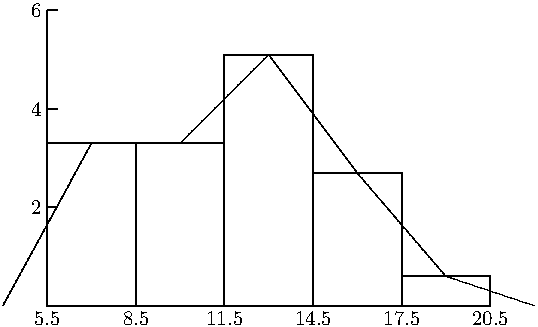
\includegraphics{histogramaarboles}


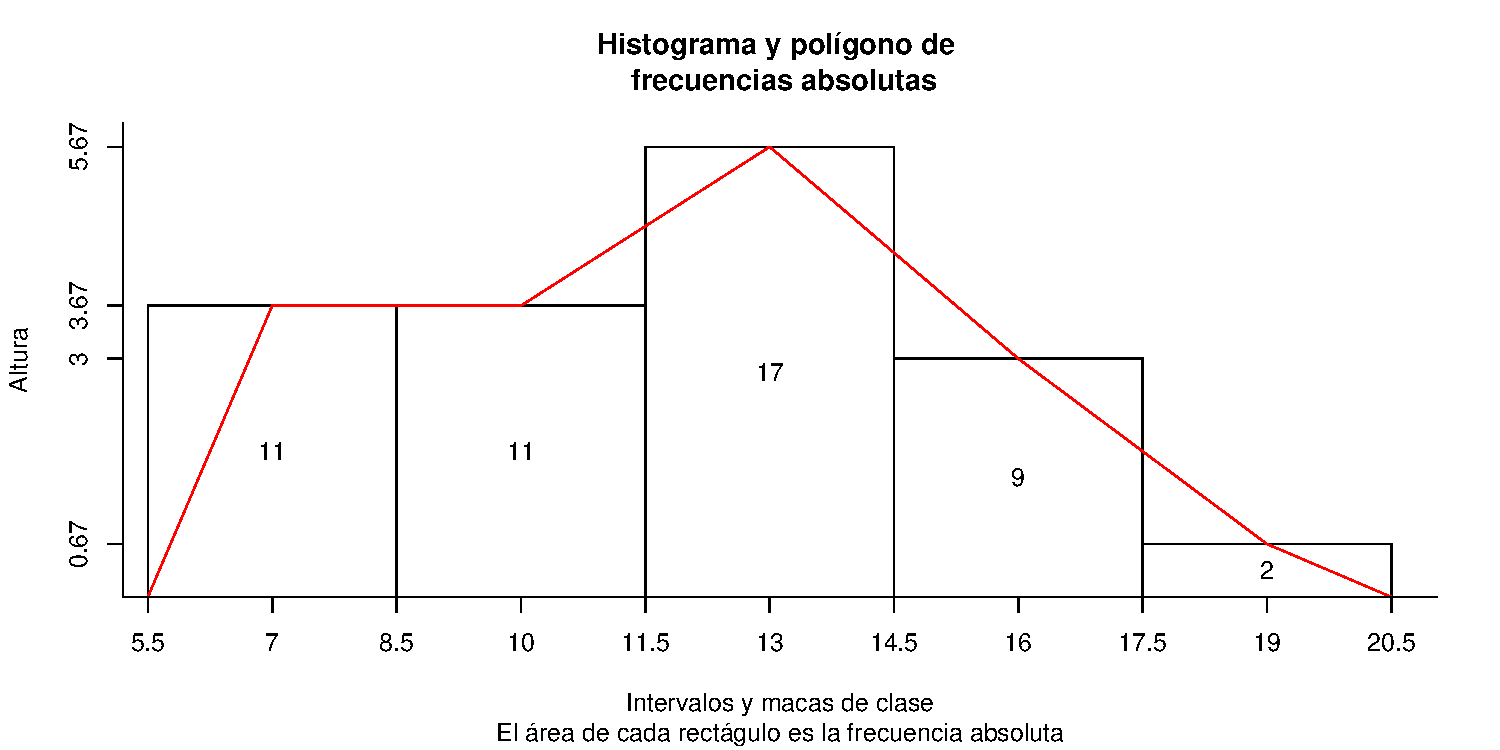
\includegraphics{./dibujos/01/-007}
\end{center}
 \caption{Histograma de frecuencias absolutas de los árboles frutales.} \label{EXEMPLE2}
\end{figure}
\label{PUNTUACIONS}
\end{frame}

\begin{frame}[fragile]
\frametitle{Distintos algoritmos de agrupamiento}
\begin{itemize}
\item La instrucción básica para agrupar datos en \texttt{R} es \texttt{cut(datos,breaks,right=F)}.
\item  Donde \texttt{datos} es el vector de datos.
\item El parámetro \texttt{breaks} (cortes) es el vector de limites de los intervalos de clase.
\item Y  \texttt{right=F} es un parámetro lógico puesto a FALSE, para indicar que los intervalos son abiertos a derecha.
\end{itemize}
\end{frame}

\begin{frame}[fragile]
El código siguiente hace el recuento de frecuencias absolutas, tal y como lo hemos hecho en el ejemplo anterior:
\begin{Schunk}
\begin{Sinput}
> options(width = 60)
> frutas <- c(8, 11, 11, 8, 9, 10, 16, 6, 12, 19, 
+     13, 6, 9, 13, 15, 9, 12, 16, 8, 7, 14, 11, 
+     15, 6, 14, 14, 17, 11, 6, 9, 10, 19, 12, 11, 
+     12, 6, 15, 16, 16, 12, 13, 12, 12, 8, 17, 
+     13, 7, 12, 14, 12)
> L <- c(5.5, 8.5, 11.5, 14.5, 17.5, 20.5)
> table(cut(frutas, breaks = L))
\end{Sinput}
\begin{Soutput}
  (5.5,8.5]  (8.5,11.5] (11.5,14.5] (14.5,17.5] (17.5,20.5] 
         11          11          17           9           2 
\end{Soutput}
\end{Schunk}

\end{frame}

\begin{frame}[fragile]
Pero si pedimos \texttt{breaks=5}  el recuento de frecuencias absolutas agrupadas puede ser distinto:
\begin{Schunk}
\begin{Sinput}
> options(width = 60)
> frutas <- c(8, 11, 11, 8, 9, 10, 16, 6, 12, 19, 
+     13, 6, 9, 13, 15, 9, 12, 16, 8, 7, 14, 11, 
+     15, 6, 14, 14, 17, 11, 6, 9, 10, 19, 12, 11, 
+     12, 6, 15, 16, 16, 12, 13, 12, 12, 8, 17, 
+     13, 7, 12, 14, 12)
> table(cut(frutas, breaks = 5))
\end{Sinput}
\begin{Soutput}
(5.99,8.59] (8.59,11.2] (11.2,13.8] (13.8,16.4]   (16.4,19] 
         11          11          13          11           4 
\end{Soutput}
\end{Schunk}
\end{frame}

\begin{frame}[fragile]
Lo mismo sucede si no modificamos las opciones del histograma:
\begin{Schunk}
\begin{Sinput}
> options(width = 60)
> frutas <- c(8, 11, 11, 8, 9, 10, 16, 6, 12, 19, 
+     13, 6, 9, 13, 15, 9, 12, 16, 8, 7, 14, 11, 
+     15, 6, 14, 14, 17, 11, 6, 9, 10, 19, 12, 11, 
+     12, 6, 15, 16, 16, 12, 13, 12, 12, 8, 17, 
+     13, 7, 12, 14, 12)
> hist(frutas)
\end{Sinput}
\end{Schunk}

\end{frame}



\begin{frame}[fragile]
\begin{figure}
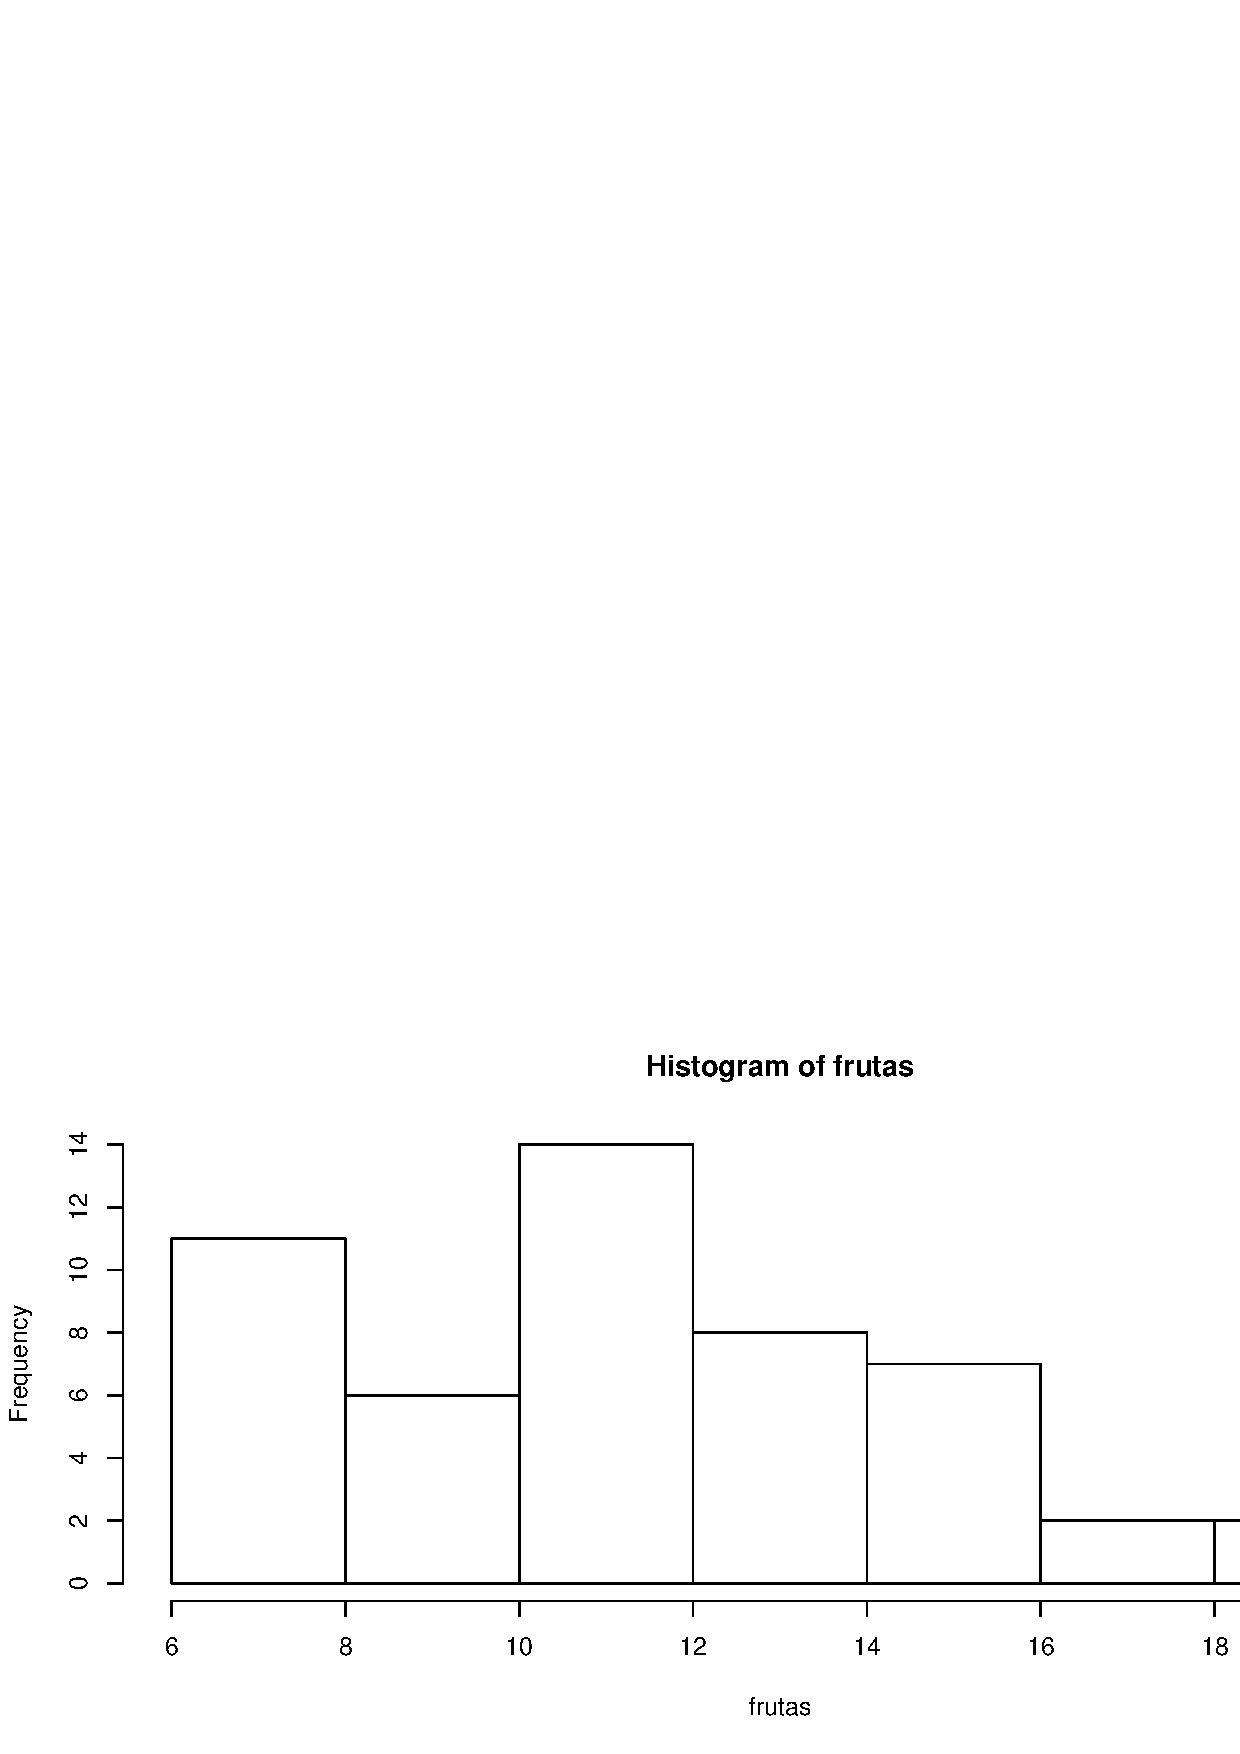
\includegraphics{./dibujos/01/-011}
\caption{Otro histograma de las frecuencias absolutas de los árboles frutales}
\end{figure}
\end{frame}

\begin{frame}
\frametitle{Mismos nombres distintos resultados}
\begin{itemize}
\item Hemos visto que los algoritmos de agrupamiento y la forma de dibujar histogramas pueden ser distintas.
\item Esto es debido a que hay varias maneras de agrupar datos.
\item Respecto a los histogramas, se suelen confundir con los diagramas de barras.
\item De hecho el concepto de histograma, como pone la ayuda de \texttt{R} para la función \texttt{hist} puede diferir según el idioma.
\item Si el objetivo del histograma es averiguar el perfil de las frecuencias, debemos usar un histograma en el que las áreas representen a las frecuencias.
\item Si todos los intervalos de clase son de la misma amplitud  el histograma de áreas o de alturas es similar. En caso contrario pueden dar severas distorsiones. 
\end{itemize}
\end{frame}


\begin{frame}[fragile]

%<<fig=FALSE,echo=TRUE>>=
\begin{Schunk}
\begin{Sinput}
> options(width = 55)
> frutas <- c(8, 11, 11, 8, 9, 10, 16, 6, 12, 
+     19, 13, 6, 9, 13, 15, 9, 12, 16, 8, 7, 
+     14, 11, 15, 6, 14, 14, 17, 11, 6, 9, 10, 
+     19, 12, 11, 12, 6, 15, 16, 16, 12, 13, 
+     12, 12, 8, 17, 13, 7, 12, 14, 12)
> L <- c(5.5, 8.5, 11.5, 14.5, 17.5, 20.5)
> h <- hist(frutas, breaks = L, main = "Hist. freq. abs.", 
+     sub = "Este histograma es la salida estándar de R", 
+     xlab = "Intervalos", ylab = paste("Frec. abs.", 
+         expression(n[i])))
> lines(c(min(h$breaks), h$mids, max(h$breaks)), 
+     c(0, h$counts, 0), type = "l", col = "red")
\end{Sinput}
\end{Schunk}

Produce la fig.~\ref{histofruta}.
\end{frame}


\begin{frame}[fragile]
\begin{figure}
\label{histofruta}
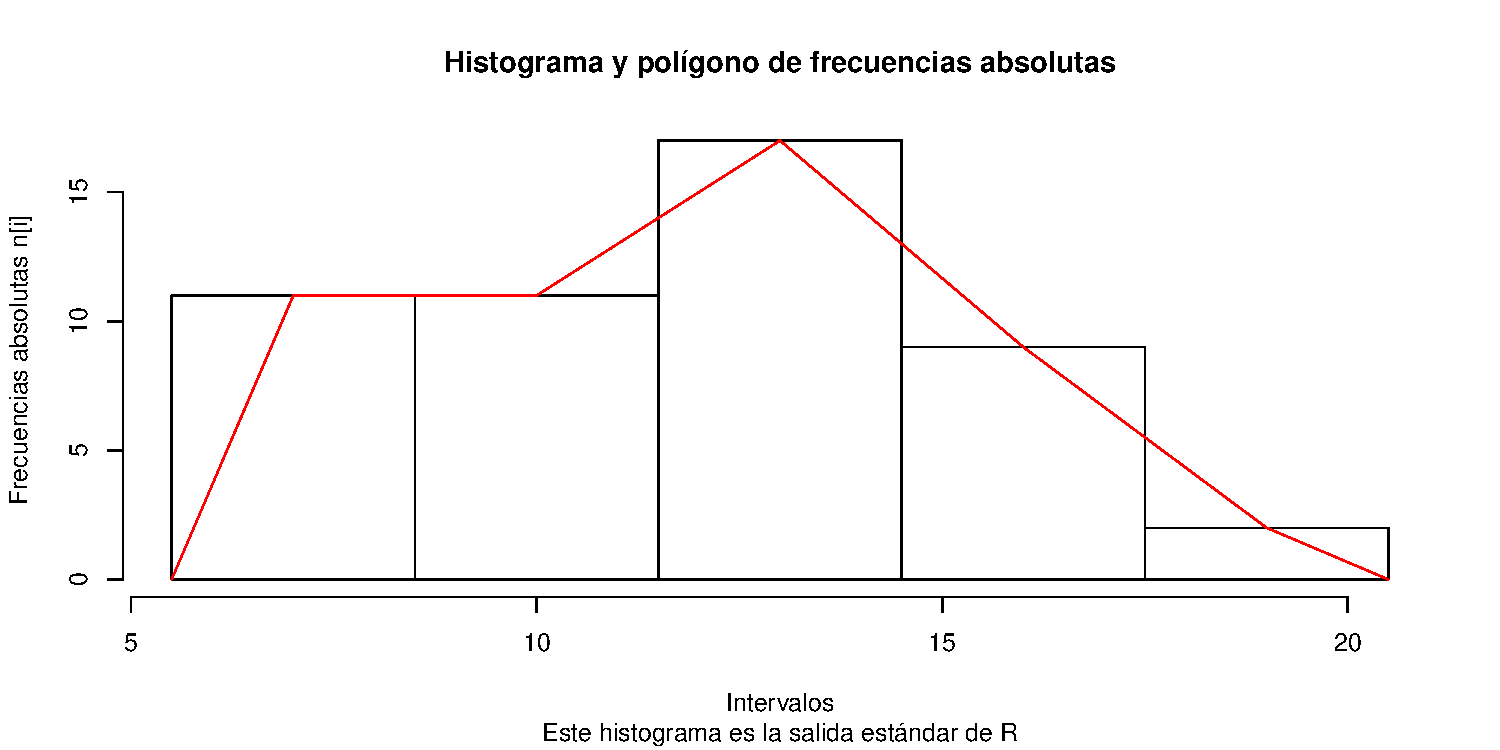
\includegraphics{./dibujos/01/-013}
\caption{Histograma (real) de los datos de árboles frutales}

Como se ve dibuja el histograma de una forma diferente (ejercicio comentar).
\end{figure}
\end{frame}

\begin{frame}
\frametitle{Datos brutos, datos agregados.}
\begin{itemize}
\item Se habla de datos brutos, micro datos,... cuando disponemos de  los datos originales  sin ningún tratamiento  informático ni estadístico.
\item Se habla de datos agregados, elaborados,... cuando los datos han  sufrido algún proceso, como el de agrupamiento.
\item Como responsables de tratar los datos podemos disponer de los datos brutos, agrupados o de ambos. 
\item  Los estadísticos básicos de los datos se calculan en  cada situación de forma  diferente y en ocasiones de ¡varias formas!
\end{itemize}
\end{frame}

\begin{frame}
\frametitle{Principales estadísticos para datos agrupados}

Ya vimos como se calculaban los principales estadísticos para datos brutos (sin agrupar). Veamos cómo se calculan para datos agrupados:

\begin{itemize}
\item Los estadísticos $\overline{x}$, $s^2$, $\tilde{s}^2$, $s$, $\tilde{s}$, se calculan  con las mismas fórmulas para frecuencias absolutas y relativas que para datos  brutos.
\item  La diferencian es que para datos brutos los valores $X_j$ son los  valores que se observan en los datos y para datos agrupados los valores $X_j$ son las marcas de clase.
\end{itemize}
\end{frame}

\begin{frame}
\begin{itemize}
\item Los estadísticos básicos pueden tener distintos valores cuando se calculan desde datos brutos o desde datos agrupados. Esto es debido a que  el tratamiento agrupado puede tener menos precisión que el de los datos brutos.
\item Esto no es en general un demérito para agrupar los datos. Es muy posible que los datos  agrupados  den más significado a la interpretación de los datos brutos.
%%explicar los de todas las frecuencias =1
\item Cuando tenemos intervalos de clase se dice \textbf{intervalo modal} al que alcanza mayor frecuencia absoluta o relativa.
\item Existen fórmulas de aproximación de la moda  para datos agrupados. No las veremos pues creemos que  carecen de interés en este curso.
\end{itemize}
\end{frame}

\begin{frame}
\frametitle{Principales estadísticos para datos agrupados}
\begin{itemize}
\item  Respecto a los gráficos ya hemos hablado de los histogramas.
\item  Comentar sobre los histogramas que no es en general admisible que  encontremos clases con frecuencia nula.
\item  Salvo comportamientos patológicos, como la existencia de dos poblaciones muy diferentes, es extraño encontrarse clases vacías. Esto suele pasar si el número de datos es pequeño y su varianza es grande.
\item En principio es aconsejable unir las clases vacías a una de sus clases contiguas.
\item Respecto a los cuantiles para datos agrupados sí hay una manera (tradicionalmente estándar)  de cálculo que expondremos más adelante.
\end{itemize}
\end{frame}



\begin{frame}
\frametitle{Ejemplo: Estadísticos de datos brutos y agrupados}
Para ilustrar las diferencias entre los estadísticos para datos brutos y agrupados
consideremos los siguientes datos:
\begin{center}
\begin{tabular}{cccccccccc}
10 & 5 & 2 & 7 & 9 & 5 & 7 & 6 & 5 & 9 \\ 12 & 2 & 6 & 6 & 9 & 12 & 6 & 6 & 6 & 4 \\
 9 & 7 & 12 & 11 & & & & & &
\end{tabular}
\end{center}

 La media aritmética de los datos anteriores sin agrupar en intervalos es:

$$\overline{x}= \frac{10+5+2+\cdots +12+11}{24}=\frac{173}{24}=7.20833$$
\end{frame}

\begin{frame}
%\frametitle{Ejemplo: Estadísticos de datos brutos y agrupados}
Si los agrupamos en intervalos de amplitud $3$, la media será (hacemos primero la
correspondiente tabla de frecuencias)
\begin{center}
\begin{tabular}{lccc}
intervalos    & $X_j$ & $n_j$ & $n_jX_j$ \\ \hline $[1.5,4.5)$   &  \ 3 &  \ 3 &   \ 9 \\
\hline $[4.5,7.5)$   &  \ 6  & 12 &  72 \\ \hline $[7.5,10.5)$  &  \ 9 &  \ 5 &  45 \\
\hline $[10.5,13.5)$ & 12  &  \ 4 &  48 \\ \hline\hline
  Suma        &   & 24   & 174
\end{tabular}
\end{center}

$$\overline{x}= \frac{174}{24}=7.25$$
Notemos que los valores difieren del de los datos brutos ya que el agrupamiento provoca una pérdida de
precisión.
\end{frame}


\begin{frame}
\frametitle{Ejemplo estadísticos datos agrupados}
% Una vez estudiadas las medidas de posición, vamos a estudiar algunos estadísticos
% que miden lo separadas que están las observaciones entre sí.

Consideremos la siguiente distribución de frecuencias

\begin{center}
\begin{tabular}{l|r|r|r|}
intervalos    & $X_j$ & $n_j$ & $n_jX_j$ \\ \hline $[9.5,29.5)$   & 19.5 &  38 &   741.0
\\ $[29.5,49.5)$  & 39.5 &  18 &   711.0 \\ $[49.5,69.5)$  & 59.5 &  31 & 1844.5 \\
$[69.5,89.5)$  & 79.5 &  20 &  1590.0   \\ \hline
    Sumas      &      & 107 &  4886.5
\end{tabular}
\end{center}
\end{frame}

\begin{frame}
\begin{itemize}
\item Vamos a calcular la varianza, primero necesitamos calcular la media $\overline{x}=\frac{4886.5}{107}=45.6682$.
\item Para calcular la varianza hemos de añadir dos columnas a la tabla anterior
\end{itemize}
\begin{center}
\begin{tabular}{crr}
 $X_j$ & $X_j^2$ & $n_jX_j^2$ \\
\hline
 19.5  & 380.25  & 14449.50 \\
 39.5  & 1560.25 &  28084.50 \\
 59.5  & 3540.25 & 109747.75 \\
 79.5  & 6320.25 & 126405.00 \\
\hline Suma   &          & 278686.75
\end{tabular}
\end{center}
 La varianza y la desviación  típica valen $s_X^2=\frac{278686.75}{107}-45.6682^2=518.962 \qquad s_X=\sqrt{518.962}=22.7807$.
\end{frame}



\begin{frame}
\frametitle{Cuantiles para datos agrupados}
\begin{itemize}
\item Veamos alguna manera de
cálculo aproximado de la mediana ($Q_{0.5}$) a partir de las frecuencia de los datos agrupados.
\item Necesitaremos las columnas de frecuencias absolutas y la de frecuencias absolutas
acumuladas para los datos agrupados.
\end{itemize}

\end{frame}

\begin{frame}
%\frametitle{Cuantiles para datos agrupados}
En general una tabla de frecuencias agrupadas es:

\begin{center}
\begin{tabular}{l|ccc|}
intervalos & $X_j$ & $n_j$ &$ N_j$ \\ \hline \hline $[L_1, L_2)$ & $X_1$ & $n_1$ & $N_1$
\\ $[L_2, L_3)$ & $X_2$ & $n_2$ & $N_2$ \\ \hline $\vdots$ & $\vdots$ & $\vdots$ &
$\vdots$ \\ \hline $[L_I, L_{I+1})$ & $X_I$ & $n_I$ & $N_I$ \\ \hline $\sum$ & & $n$ &
\end{tabular}
\end{center}
\end{frame}

\begin{frame}
\begin{itemize}
\item Llamaremos intervalo crítico para la mediana al primer intervalo en el que su frecuencia
absoluta acumulada supere o iguale a $\frac{n}{2}$.
\item  Denotemos por $[L_c, L_{c+1})$  el
intervalo crítico.
\item  Sea $N_{c-1}$ la frecuencia absoluta acumulada del intervalo anterior
al crítico.
\item  En el caso en que el intervalo crítico sea  el primero, $N_{c-1}=0$.
\item  Sea $n_c$
la  frecuencia absoluta del intervalo crítico. 
\item Sea  $A_c=L_{c+1}-L_c$ la amplitud del
intervalo crítico. 
\item Una  aproximación para la \textbf{mediana}  la da la siguiente fórmula:
$$Q_{0.5}=L_{c}+A \frac{\left(\frac{n}{2}- N_{c-1}\right)}{n_c}.$$
\end{itemize}
\end{frame}

\begin{frame}
\frametitle{Cuantiles para datos agrupados}
\begin{itemize}
\item La justificación de la fórmula anterior es la siguiente.
\item  Si representásemos las frecuencias absolutas acumuladas entre los extremos de los intervalos, la mediana seria
la antiimagen de $\frac{n}{2}$ en  el intervalo crítico haciendo una interpolación por
lineal (ver figura~\ref{MEDIANA}).
\end{itemize}
\end{frame}

\begin{frame}
\begin{figure}
\begin{center}
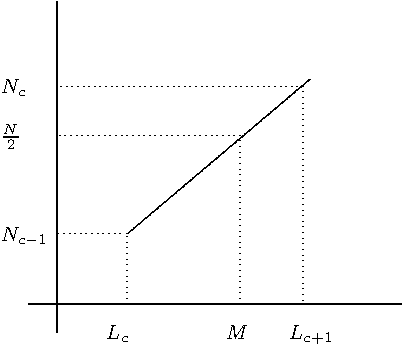
\includegraphics[scale=0.6]{interpretacion}
\end{center}
\caption{Interpretación geométrica de la Mediana} \label{MEDIANA}
\end{figure}
\end{frame}

\begin{frame}
\begin{itemize}
\item Los cuantiles son una generalización de la mediana. La mediana es el cuantil $0.5$ ya
que deja el 50\% de las observaciones a su izquierda.
\item En general el \textbf{cuantil}~$p$ es aquel valor que deja el~$p\cdot 100\%$ de las
observaciones a su izquierda. Por  lo tanto el cuantil $p$ es $Q_{p}$.
El cálculo, dada la distribución de frecuencias es semejante al cálculo de la mediana.
\item Definimos el  intervalo crítico  en  este caso  como el primer intervalo del que su
frecuencia absoluta acumulada supera o iguala a $n\cdot p$.
\end{itemize} 
\end{frame}

\begin{frame}
\begin{itemize}
\item Sean entonces, $[L_c, L_{c+1})$ el intervalo crítico,  $N_{c-1}$ la frecuencia absoluta acumulada del intervalo anterior al crítico y  $n_c$ la frecuencia absoluta del intervalo crítico.
\item  Si denotamos por  $A_c$ a la amplitud  del intervalo crítico, la fórmula para calcular el  \textbf{cuantil}~$p$ es: $Q_{p} =L_c + A_c \frac{\left(n\cdot p-N_{c-1}\right)}{n_c}.$
\end{itemize}
\end{frame}

\begin{frame}
\frametitle{Ejemplo del cálculo de la mediana.}
Calculemos la mediana, sin agrupar,  de los siguientes datos:

$$
14, 15, 16, 18, 18, 18, 18, 19, 20, 20, 22.
$$
El tamaño de la muestra es $n=11$ observaciones y ya están ordenadas. El lugar central,
es el que ocupa  el sexto puesto, el valor que ocupa este lugar es el $18$, por lo tanto,
la mediana es $18$.
\end{frame}

\begin{frame}
En la siguiente muestra tenemos un número par de datos:
$$
24, 25, 26, 26, 27, 27, 27, 29.
$$
El tamaño muestral es $n=8$ observaciones que ya están ordenadas. El lugar central estará
entre el  cuarto y el quinto puesto. Los datos que ocupan estos lugares son el $26$ y el
$27$. Por lo tanto la mediana vale

$$Q_{0.5}=\frac{26+27}{2}=26.5.$$
\end{frame}

\begin{frame}

\frametitle{Ejemplo}
Consideremos la siguiente  distribución de frecuencias: {\rm
$$
\begin{tabular}{lccc}
intervalos &  $X_j$ &  $n_j$ &  $N_j$ \\ \hline $[1.5,4.5)$   & \ 3  &  \ 3 &   \ 3  \\
$[4.5,7.5)$   & \ 6  & 12 &  15  \\ $[7.5,10.5)$  & \ 9  &  \ 5 &  20  \\ $[10.5,13.5)$ &
12 &  \ 4 &  24  \\ \hline
\end{tabular}
$$
} Tenemos  que $n=24$ y que  $\frac{n}{2}=12$. El intervalo crítico es:
 $[4.5,7.5)$
\end{frame}

\begin{frame}
La mediana valdrá entonces:

$$Q_{0.5}=4.5+3\frac{(12-3)}{12}=6.75.$$

Cuantil $0.25$: $25\mbox{\%}\Rightarrow  n\cdot p= 6$. Intervalo crítico:
 $[4.5,7.5)$.

$$Q_{0.25}=4.5+3\frac{(6-3)}{12}=5.25$$

Cuantil $0.75$: $75\mbox{\%} \Rightarrow  n\cdot p= 18$. Intervalo crítico:
 $[7.5,10.5)$.

$$
Q_{0.75}=7.5+3\frac{(18-15)}{5}=9.3
$$
\end{frame}

\begin{frame}
\begin{itemize}
\item Los cuartiles
que dividen a la población en cuartos son llamados cuartiles, así el primer cuartil $Q_{0.25}$
deja a su izquierda el 25\% de las observaciones, el segundo cuartil $Q_{0.5}$ es la mediana
y el tercer cuartil $Q_{0.75}$ deja a su izquierda el $75\%$ de las observaciones.
\item  También se
habla de los deciles que son los estadísticos que dividen a la población en décimas
partes: $Q_{0.1}, Q_{0.2},\ldots$.
\item Los percentiles son los que dividen la muestra en centésimas partes.
\end{itemize}
\end{frame}

\subsection{Cambios de escala y de origen}

\begin{frame}
\frametitle{Cambios lineales}
\begin{itemize}
\item Supongamos que tenemos una serie de datos $x_1,x_2,\ldots,x_n$ de una variable $X$.
\item Les vamos a realizar una transformación lineal $Y=a\cdot X+b$.
\item Obtendremos la serie de datos $y_1=a \cdot x_1+b,\quad y_2=a \cdot x_2+b,\ldots, y_n=a \cdot x_n+b$.
\item La pregunta es ¿cómo afecta esta operación a los estadísticos básicos?
\item Denotaremos por $\overline{x}$, $s_X^2$, a la media y la varianza de los datos $X$ y  denotaremos por $\overline{y}$  y $s_y^2$
a la media y la varianza de los datos de la  variable $Y$.
\end{itemize}
\end{frame}


\begin{frame}
\frametitle{Interpretación cambios lineales}
\begin{itemize}
\item Si $b>0$ los datos se desplazan su origen en una cantidad $b$ a su derecha.
\item Si $b<0$ los datos se desplazan su origen en una cantidad $b$ a su izquierda.
\item Por esto motivo sumar una cantidad $b$ recibe el nombre de \textbf{cambio de origen}.
\item Si $a\geq 1$ las unidades de los datos aumenta su escala en esa proporción.
\item Si $0<a<1$ los datos reducen su escala es esa proporción.
\item Si $a<0$ la interpretación es similar salvo porque los datos sufren también un cambio de orientación.
\item Es por esos motivos por lo que multiplicar los datos por una cantidad $a$ recibe el nombre de \textbf{cambio de escala}.
\end{itemize}
\end{frame}


\begin{frame}
Se cumplen  las siguientes propiedades:
\begin{itemize}
\item La media queda afectada de   la misma forma que los datos por el cambio lineal.
\item Es decir $\overline{y}= a \cdot \overline{x}+b$.
\item La varianza es independiente respecto a  cambios de origen y que
queda afectada por el cuadrado de los cambios de escala.
\item Es decir  $s_Y^2 = a^2 s_X^2.$
\item Para las desviaciones típicas tendremos $$s_Y=|a| s_X.$$
\end{itemize}
\end{frame}


% \begin{frame}
% \begin{itemize}
% \item La media queda afectada de   la misma forma que los datos por el cambio lineal.
% \item Es decir $\overline{y}= a \cdot \overline{x}+b$.
% \item De aquí deducimos que la varianza es independiente respecto a  cambios de origen y que
% queda afectada por el cuadrado de los cambios de escala.
% \item Es decir  $s_Y^2 = a^2 s_X^2.$
% \item Para las desviaciones típicas tendremos $$s_Y=|a| s_X.$$
% \end{itemize}
% \end{frame}
% 


\begin{frame}
\frametitle{Puntuaciones típicas}
\begin{itemize}
\item Consideremos los datos de una variable $X$, $x_1,x_2,\ldots,x_n$ de los que conocemos $\overline{x}$ y $s_X$. Consideremos el cambio lineal, o de escala y origen, $Z=\frac{X-\overline{x}}{s_X}$.
\item La  puntuaciones $z_1=\frac{x_1-\overline{x}}{s_X},z_2=\frac{x_2-\overline{x}}{s_X},\ldots, z_n=\frac{x_n-\overline{x}}{s_X}$
reciben el nombre de puntuaciones típicas o tipificadas o estándar  de los datos $X$.
\item Estas puntuaciones cumplen que $\overline{z}=0$ y $s_z=1$. Es decir transformamos los datos a unos datos que tienen media cero y varianza 1.
\item Las puntuaciones típicas, entre otras cosas,  son útiles para comparar distribuciones de frecuencias de dos o más  variables medidas en distintas unidades.
\end{itemize}
\end{frame}








\begin{frame}
\frametitle{Ejemplo de datos agrupados}
% Una vez estudiadas las medidas de posición, vamos a estudiar algunos estadísticos
% que miden lo separadas que están las observaciones entre sí.

Consideremos la siguiente distribución de frecuencias

\begin{center}
\begin{tabular}{lrrr}
intervalos    & $X_j$ & $n_j$ & $n_jX_j$ \\ \hline $[9.5,29.5)$   & 19.5 &  38 &   741.0
\\ $[29.5,49.5)$  & 39.5 &  18 &   711.0 \\ $[49.5,69.5)$  & 59.5 &  31 & 1844.5 \\
$[69.5,89.5)$  & 79.5 &  20 &  1590.0   \\ \hline
    Suma     &      & 107 &  4886.5
\end{tabular}
\end{center}
\end{frame}

\begin{frame}
\begin{itemize}
\item Vamos a calcular la varianza, primero necesitamos calcular la media $\overline{x}=\frac{4886.5}{107}=45.6682$.
\item Para calcular la varianza hemos de añadir dos columnas a la tabla anterior
\end{itemize}
\begin{center}
\begin{tabular}{crr}
 $X_j$ & $X_j^2$ & $n_jX_j^2$ \\
\hline
 19.5  & 380.25  & 14449.50 \\
 39.5  & 1560.25 &  28084.50 \\
 59.5  & 3540.25 & 109747.75 \\
 79.5  & 6320.25 & 126405.00 \\
\hline Suma   &          & 278686.75
\end{tabular}
\end{center}
 La varianza y la desviación  típica valen $s_X^2=\frac{278686.75}{107}-45.6682^2=518.962 \qquad s_X=\sqrt{518.962}=22.7807$.
\end{frame}

\section{Más estadísticos}
\subsection{Coeficiente de variación}

\begin{frame}
\frametitle{Ejemplo de datos agrupados}
\begin{itemize}
\item  El coeficiente de variación  se define como el cociente entre la desviación típica  y la media aritmética.
\item  Se utiliza para variables en las que la media represente a la magnitud de los
datos. Esto sucede cuando por ejemplo todos son positivos.
\item La notación y fórmula para el cálculo es $CV=\frac{s}{\overline{x}}.$
\end{itemize}
\end{frame}

\begin{frame}
\begin{itemize}
\item  El coeficiente de variación  es independiente del cambio de escala. 
\item Más concretamente, consideremos  el cambio lineal  de la variable $X$ $Y=a X$, con $a>0$,  el coeficiente de
variación  de la variable $Y$ es el mismo que el de la variable $X$:
$$CV_Y=CV_X.$$
\item El coeficiente de variación será útil para comparar la dispersión de distribuciones
 de frecuencias de dos o más variables en diferentes escalas.
\end{itemize}
\end{frame}

\begin{frame}
\frametitle{Ejemplo}
Consideremos la siguiente distribución de frecuencias: 
\begin{center}
\begin{tabular}{lccc}
intervalos     & $X_j$ & $n_j$ & $n_jX_j$\\ \hline $[9.5,29.5)$  & 19.5 & \ 38  & \ 741.0
\\ $[29.5,49.5)$ & 39.5 & \ 18  & \ 711.0  \\ $[49.5,69.5)$ & 59.5 & \ 31  & 1844.5 \\
$[69.5,89.5)$ & 79.5 & \ 20  & 1590.0   \\ \hline Sumas     &      & 107 & 4886.5
\end{tabular}
\end{center}
\end{frame}

\begin{frame}
\frametitle{Ejemplo}
\begin{itemize}
\item La media   y la desviación  típica son $\overline{x}=45.6682,\quad s_X=22.7807$.
\item Por lo tanto el coeficiente de variación es $CV=\frac{s}{\overline{x}}=\frac{22.6807}{45.6682}=0.4988$.
\end{itemize}
\end{frame}

\begin{frame}
\frametitle{Perfil de una distribución}
\begin{itemize} 
\item El perfil de una distribución viene determinado por alguno de sus polígonos de
frecuencias. 
\item Es mejor utilizar las frecuencias relativas ya que no dependen del tamaño de
la muestra. 
\item La idea es encontrar la curva la que tiende el polígono de frecuencias
cuando la muestra se hace grande, que en definitiva sería la curva de frecuencias de toda
la población.
\end{itemize}
\end{frame}

\begin{frame}
\begin{figure}
\begin{center}
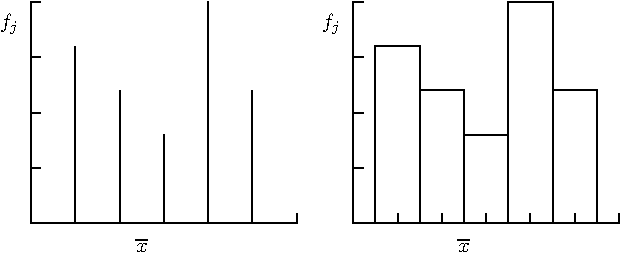
\includegraphics{diagrama}
\end{center}
\caption{Diagrama de barras e  histograma de las frecuencias relativas }
\label{RELATIVES}
\end{figure}
\end{frame}

\begin{frame}
\frametitle{El perfil de una distribución}
\begin{itemize}
\item Una curva continua en forma de campana llamada curva de Gauss. Puede servir como un modelo
matemático ideal para comparar el perfil de cualquier distribución.
\item  Esta curva
corresponde a la gráfica de la función
$$y=\frac{1}{\sigma\sqrt{2\pi}} e^{-\frac{(x-\mu)^2}{2\sigma^2}},$$
\item Donde  $\mu$ se aproxima por $\overline{x}$  y  $\sigma$ por $s$.
\item Su representación gráfica es la de la figura~\ref{NORMAL}, gaussiana o campana de gauss, para el caso (estándar) en el  que~$\mu=0$ y~$\sigma =1$.
\end{itemize}
\end{frame}

\begin{frame}
\frametitle{La campana de gauss}
\begin{figure}
\begin{center}
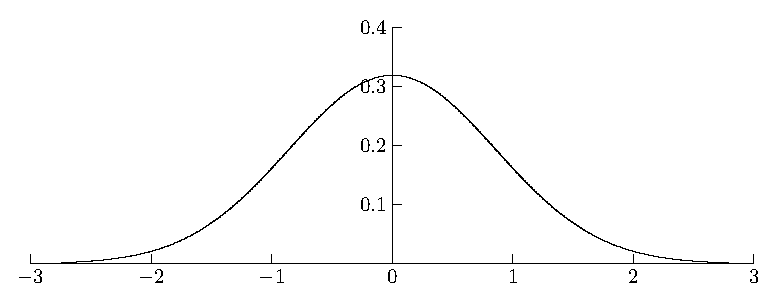
\includegraphics{curva}
\end{center} \caption{Curva normal o campana de Gauss} \label{NORMAL}
\end{figure}
\end{frame}

\begin{frame}
\frametitle{Propiedades de la curva normal}
Las propiedades más importantes de la curva normal son:
\begin{enumerate}[a)]
\item Está definida para cualquier real  y es siempre positiva.
\item El área comprendida entre  la curva y el eje de abscisas
vale siempre $1$ para cualquier valor de $\mu$ y $\sigma>0$.
\item Es simétrica respecto a la recta vertical $X=\mu$ y en este punto
tiene un máximo absoluto que vale $\frac{1}{\sqrt{2 \pi} \sigma}$.
\item Tiene dos puntos de inflexión en $x=\mu \pm \sigma$.
\item El eje de abscisas es una asíntota de la curva.
\end{enumerate}
\end{frame}

\begin{frame}
\frametitle{La normal y las medidas de simetría y apuntamiento}
\begin{itemize}
\item Las medidas de simetría y apuntamiento se suelen referir a la correspondiente
distribución normal.
\item Es decir  aquella en la que los parámetros se estiman por  $\mu=\overline{x}$
y $\sigma=s.$ ( o por la cuasivarianza).
\item Se entiende, entonces, que la distribución normal es simétrica y es perfecta respecto 
al apuntamiento.
\item  Es decir, que no es ni apuntada ni chata.
\end{itemize}
\end{frame}

\subsection{Medidas de simetría}

\begin{frame}
\frametitle{Índice de simetría}
\begin{itemize}
\item 
Para ver si una distribución es simétrica o asimétrica por la derecha o por la izquierda
se toma como índice de simetría (\textsl{skewness}):$g_1=\frac{m_3}{s^3},$
\item Donde $m_3$ es el momento central de tercer orden y se calcula de la siguiente forma:
$m_3=\frac{1}{n}\sum\limits_{j=1}^{k} n_j(X_j-\overline{x})^3,$
\item Por supuesto, $s$ es la desviación típica.
\end{itemize}
\end{frame}

\begin{frame}
\frametitle{Índice de simetría}
Interpretación del índice de simetría:
\begin{itemize}
\item[-] Si $g_1>0$, la distribución
es asimétrica por la derecha o asimetría positiva.
\item[-] Si $g_1=0$, la distribución
es simétrica o el  índice no decide.
\item[-] Si $g_1<0$, la distribución
es asimétrica por la izquierda o asimetría negativa.
\end{itemize}
\end{frame}

\begin{frame}
%%%%%%CAMIBIAR DIBUJO INCLUIR PIES CON g1<0 g1=0 g1>0
\begin{figure}
\begin{center}
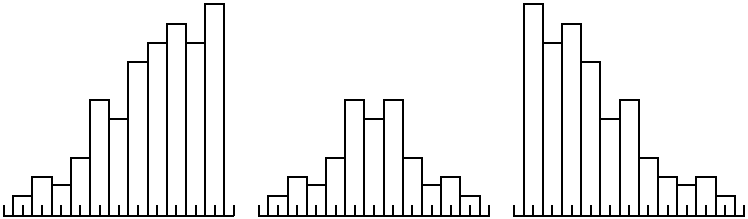
\includegraphics{histogramas2}
\end{center} 
\caption{Histogramas, de izquierda a derecha, para $g_1>0$, $g_1\approx 0$ y $g_1<0$.}
\end{figure}
\end{frame}

\begin{frame}
\frametitle{Ejemplo simetría}
Consideremos la siguiente distribución de frecuencias: 

\begin{center}
\begin{tabular}{lrrrr}
intervalos  &  $X_j$ & $ n_j$ &  $n_jX_j$  &  $n_jX_j^2$ \\ \hline $[14.5,19.5)$ & 17  &
4    & 68   & 1156  \\ $[19.5,24.5)$ & 22  &  6   & 132   & 2904
\\ $[24.5,29.5)$ & 27  &  8  &  216   & 5832 \\ $[29.5,34.5)$ & 32  & 11  &  352   &
11264 \\ $[34.5,39.5)$ & 37  & 35  & 1295   & 47915 \\ $[39.5,44.5)$ & 42  &100  & 4200 &
176400 \\ $[44.5,49.5)$ & 47  & 218 & 10246 & 481562 \\ \hline
  Suma      & &   382 & 16509 & 727033
\end{tabular}
\end{center}
\end{frame}

\begin{frame}
\frametitle{Ejemplo simetría}
\begin{itemize}
\item La media y la varianza valen: $\overline{x}=  \frac{16509}{382}=43.2173, \quad s_{X}^2=
\frac{727033}{382}-\left(\frac{16509}{382}\right)^2=35.49$
\item Calculemos el  coeficiente de simetría $g_1$.  Para hacerlo, hemos de añadir una columna
más a la tabla anterior.
\end{itemize}
\end{frame}

\begin{frame}
\frametitle{Ejemplo simetría}
\begin{center}
\begin{tabular}{rrr}
        $X_j$ &  $ n_j$ &    $n_j {(X_j-\overline{x})}^3$ \\
\hline
        17 &   4  & -72081.33  \\
        22  &  6  & -57308.66 \\
        27  &  8  & -34121.16 \\
        32  & 11  & -15525.84 \\
        37  & 35  &  -8411.41 \\
        42  & 100  &  -180.37 \\
        47  & 218  & 11799.67 \\
\hline
 Sumas       & 382  &-175829.09
\end{tabular}
\end{center}
\end{frame}

\begin{frame}
\frametitle{Ejemplo simetría}
\begin{itemize}
\item El momento de tercer orden vale $m_3=\frac{-175829.09}{382}=-460.285$.
\item Calculemos el índice de simetría $g_1=\frac{m_3}{s^3}=\frac{-460.285}{\left(\sqrt{35.49}\right)^3}=-2.18$.
\item Por lo tanto podemos decir que se trata de una distribución asimétrica por la izquierda o
negativa.
\end{itemize}
\end{frame}



\subsection{Medidas de apuntamiento}

\begin{frame}
\frametitle{Medidas de apuntamiento para datos numéricos}
\begin{itemize}
\item Las medidas de apuntamiento nos miden si el perfil de una distribución muestral está muy
apuntado o no en comparación con un perfil ideal.
\item EL modelo ideal  es el de la campana de
gauss asociada.
\item  Para estudiar el apuntamiento se utiliza un índice basado en el momento
de cuarto orden, que recibe el nombre de coeficiente de apuntamiento o curtosis (\textsl{kurtosis}.)
\end{itemize}
\end{frame}

\begin{frame}
\begin{itemize}
\item La fórmula de la curtosis es
$$g_2=\frac{m_4}{s^4}-3,$$
\item Donde $m_4$ es el llamado momento central de cuarto orden y se calcula de la
siguiente forma:
$$
m_4 =\frac{1}{n} \sum\limits_{j=1}^{k} n_j(X_j - \overline{x})^4,
$$
\item Donde  $s$  es la desviación típica.
\end{itemize}
\end{frame}

\begin{frame}
\frametitle{Medidas de apuntamiento para datos numéricos}
 Tenemos, pues  que:
\begin{itemize}
\item[-] Si  $g_2>0$, la distribución
es puntiaguda o leptocúrtica.
\item[-]Si $g_2=0$, la distribución
es similar a la normal o mesocúrtica.
\item[-] Si $g_2<0$, la distribución
es achatada o platicúrtica.
\end{itemize}
\end{frame}
\begin{frame}
\frametitle{Medidas de apuntamiento para datos numéricos}
La siguiente figura ilustra las diferencias entre los valores de apuntamiento.
\begin{figure}
\begin{center}
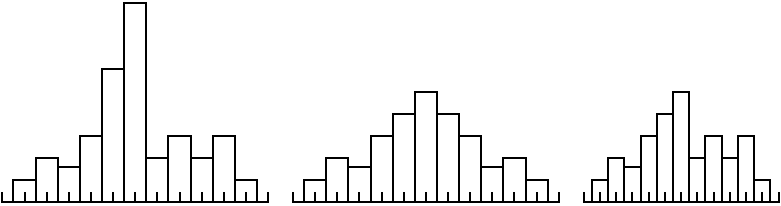
\includegraphics{histogramas3}
\end{center}
\caption{Histogramas de los tres tipos de apuntamiento}
\end{figure}
\end{frame}

\begin{frame}
\frametitle{Ejemplo apuntamiento}
Consideremos la siguiente distribución de frecuencias:
\begin{center}
\begin{tabular}{lrrrr}
intervalos  &  $X_j$  & $n_j$   & $n_jX_j$   & $n_j X_j^2$  \\ \hline $[14.5,19.5)$ & 17
& 4    & 68    & 1156  \\ $[19.5,24.5)$ & 22  & 6    & 132   & 2904
\\ $[24.5,29.5)$ & 27 &   8   & 216   & 5832 \\ $[29.5,34.5)$ & 32 &  11   & 352   &
11264 \\ $[34.5,39.5)$ & 37 &  35   & 1295  &  47915 \\ $[39.5,44.5)$ & 42 & 100   & 4200
& 176400 \\ $[44.5,49.5)$ & 47 & 218  & 10246  & 481562 \\ \hline
  Sumas     & &    382  & 16509  & 727033
\end{tabular}
\end{center}
\end{frame}


\begin{frame}
\frametitle{Ejemplo apuntamiento}
\begin{itemize}
 \item La media y la varianza valen $
\overline{x} =  \frac{16509}{382}=43.22,\quad s_X^2=
\frac{727033}{382}-\left(\frac{16509}{382}\right)^2=35.49$.
\end{itemize}
\end{frame}

\begin{frame}
\begin{itemize}
\item Calculemos coeficiente de apuntamiento $g_2$.  Hemos de añadir una columna a la tabla:
\end{itemize}
\begin{center}
\begin{tabular}{lrrr}
intervalos  &  $X_j$  & $n_j $  & $n_j(X_j-\overline{x})^4$   \\ \hline $[14.5,19.5)$ &
17 & 4    & 1889776.11 \\ $[19.5,24.5)$ & 22  & 6    & 1215933.65 \\ $[24.5,29.5)$ & 27 &
8 &  553352.38 \\ $[29.5,34.5)$ & 32 &  11   & 174157.64 \\ $[34.5,39.5)$ & 37 &  35 &
52296.07 \\ $[39.5,44.5)$ & 42 & 100   &  219.56 \\ $[44.5,49.5)$ & 47 & 218  & 44634.88
\\ \hline
  Sumas     & &    382  & 3930370.29
\end{tabular}
\end{center}
\end{frame}


\begin{frame}
\frametitle{Ejemplo apuntamiento}
\begin{itemize}
\item  El momento de cuarto orden vale $m_4=\frac{3930370.29}{382}=10288.93$.
\item Calculemos el índice de apuntamiento
$g_2=\frac{m_4}{s^4} -3 =\frac{10288.93}{35.49^2}-3=5.17$.
\item Por lo tanto se trata  de una distribución puntiaguda o leptocúrtica.
\end{itemize}
\end{frame}

\begin{frame}
\subsection{Cambios de escala y origen}
El  índice de apuntamiento es independiente respecto cambios lineales  de la forma
$Y=aX+b$, es decir:

 $$g_2(X)=g_2(Y).$$


El índice~$g_2$ no queda afectado por cambios de origen ni de escala.
\end{frame}

% \begin{frame}
% 
% Cuando  la variable $X$ se vea afectada por un cambio lineal: $Y=aX+b$, la varianza de
% $Y$ cumple la siguiente relación:
% 
% $$s_Y^2 = a^2 s_X^2.$$
% 
% De aquí deducimos que la varianza es independiente respecto a  cambios de origen y que
% queda afectada por el cuadrado de los cambios de escala.
% \end{frame}
% 
% \begin{frame}
% Para las desviaciones típicas tendremos:
% $$s_Y=|a| s_X.$$
% El índice de simetría es independiente de cambios lineales de la forma $Y=aX+b$, con
% $a>0$, es decir:
% 
% $$g_1(X)=g_1(Y).$$
% En otras palabras, el índice de simetría no queda afectado por cambios de origen, ni por
% cambios de escala positivos, mientras que para cambios de escala negativos cambia el
% signo de la simetría (ejercicio).
% \end{frame}

\begin{frame}
El coeficiente de variación  es independiente del cambio de escala. Más concretamente, si
hacemos el cambio lineal  de la variable $X$ $Y=a X$, con $a>0$,  el coeficiente de
variación  de la variable $Y$ es el mismo que el de la variable $X$:

$$CV_Y=CV_X.$$

El coeficiente de variación será útil para comparar la dispersión de distribuciones
medidas en diferentes escalas.


\end{frame}

\begin{frame}
\frametitle{El diagrama de caja}
\begin{itemize}
\item EL diagrama de caja es un gráfico que resume algunos estadísticos de una serie de datos en un gráfico.
\item Este gráfico está formado por cinco números que en orden son:
$b_{inf},Q_{0.25},Q_{0.5},Q_{0.75},b_{sup}$
\item Los valores $b_{inf},b_{sup}$ determinan los extremos o bigotes del dibujo. Si denotamos por $m$ y $M$ el mínimo y el máximo de los datos, se calculan de la siguiente forma:
$b_{inf}=\mbox{mín}\{m, Q_{0.25}-1.5\cdot\left(Q_{0.75}-Q_{0.25}\right\}$

$b_{sup}=\mbox{máx}\{M, Q_{0.75}+1.5\cdot\left(Q_{0.75}-Q_{0.25}\right\}$
\item La fig.~\ref{boxplot} explica como se dibuja el diagrama de caja (\textsl{box plot})
\end{itemize}
\end{frame}

\begin{frame}
\begin{center}
\begin{figure}\label{boxplot}
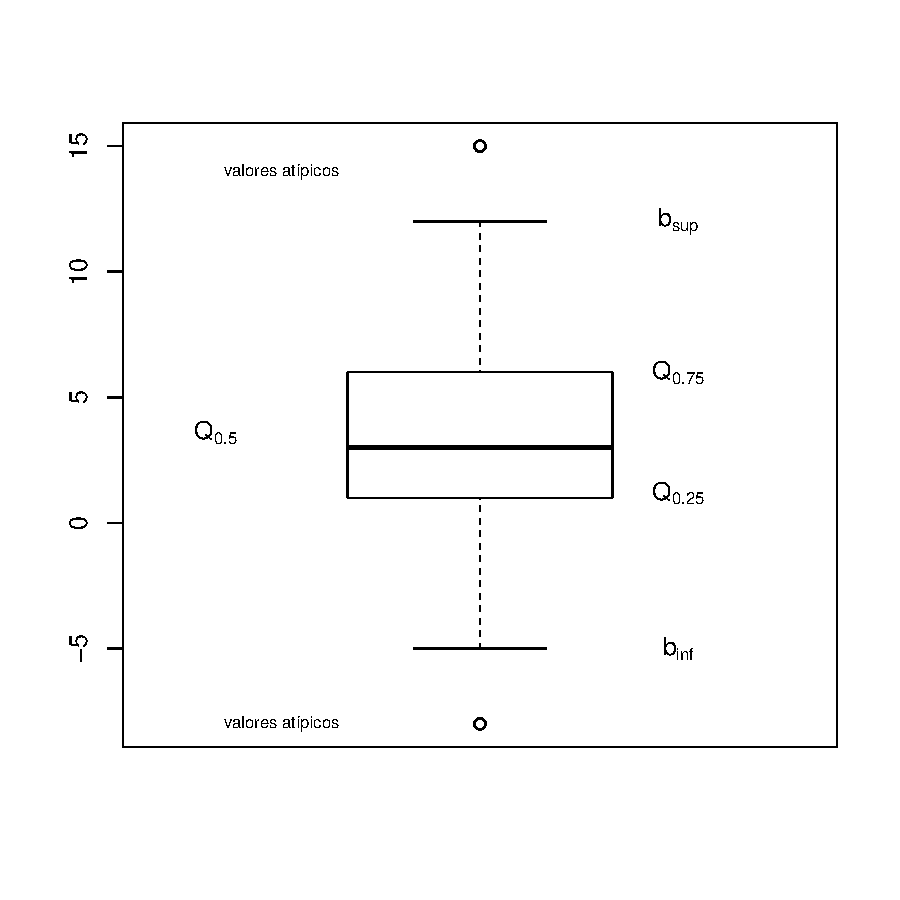
\includegraphics{./dibujos/01/-014}
\caption{Esquema para el dibujo de un diagrama de caja}
\end{figure}
\end{center}

\end{frame}



\section{Variables multidimensionales}

\begin{frame}
\frametitle{Variables multidimensionales}
\begin{itemize}
\item Hasta ahora sólo hemos estudiado una variable, es evidente que en la realidad interesa el
comportamiento conjunto de dos o más variables.
\item  En cualquier disciplina técnica o
científica, economía, ciencias de la computación, bioinformática,
telecomunicaciones,\ldots son muy utilizados los conceptos de asociación, independencia y
otros, entre dos o más variables.
\end{itemize}
\end{frame}

\begin{frame}
\frametitle{Variables multidimensionales}
\begin{itemize}
\item  Para introducirlos estudiaremos el caso más sencillo;
el de las variables estadísticas bidimensionales. En lo que respecta a esta sección cada
individuo de la población tiene asociado más de un valor o cualidad observada.
\item   Por ejemplo peso y altura de un grupo de personas, peso y sexo, altura y nivel de estudios,
\ldots. 
\end{itemize}
\end{frame}

\begin{frame}
\frametitle{Variables multidimensionales}
\begin{itemize}
\item Por ejemplo  si estudiamos el peso ($p$) y la altura ($h$) de una población una
muestra genérica de tamaño $n$ tendría el siguiente aspecto:
$$
 (p_1,h_1),(p_2,h_2),\ldots,(p_n,h_n),
$$
\item Donde  $(p_i, h_i)$ es el peso y la estatura correspondientes a la observación $i$-ésima.
\item Otro ejemplo sería el estudio de la relación entre los turistas llegados a nuestra isla y
el año de llegada.
\item  Los datos serían $(t_1,n_1),(t_2,n_2),\ldots,(t_N,n_N)$
donde $t_i$ es el año $i$-ésimo y  $n_i=$ número de turistas llegados ese año.
\end{itemize}
\end{frame}

\subsection{Descripción numérica: caso bidimensional}
\begin{frame}
\frametitle{Descripción numérica: caso bidimensional}
\begin{itemize}
\item Supongamos que tenemos $(X,Y)$  un par de variables que se pueden medir conjuntamente en
un individuo de la población que se desea estudiar.
\item Sean $\{X_1,X_2,\ldots, X_I\}$ los valores que han tomado los datos  de  $X$ y   $\{Y_1,Y_2,\ldots, Y_J\}$
los de $Y$.
\item El conjunto de valores que puede tomar la variable conjunta $(X,Y)$ son:
$
\left\{(X_1,Y_1),\ldots,(X_1,Y_J),(X_2,Y_1)\ldots\right.
$
$
\left.,(X_2,Y_J),\ldots,(X_I,Y_1),\ldots
,(X_I,Y_J)\right\}.
$.
\end{itemize}
\end{frame}

\begin{frame}
\begin{itemize}
\item Sean $n_{ij}$ la frecuencia absoluta correspondiente al valor  $(X_i,Y_j)$, o sea, es el
nombre de individuos de la muestra que tienen la variable $X$ igual a $X_i$ y la variable
$Y$ igual a $Y_j$.
\item Toda esta información se puede resumir en la siguiente tabla de frecuencias absolutas o
tabla de contingencia:
\end{itemize}
\end{frame}

\begin{frame}
\begin{center}
\begin{tabular}{|c|cccccc|c|}
\hline $X\mbox{\textbackslash} Y$ & $Y_1$ & $Y_2$ & $\ldots$ & $Y_j$ & $\ldots$ & $Y_J$ & $n_{i \bullet}$ \\
\hline $X_1$ & $n_{11}$ & $n_{12}$ & $\ldots$ & $n_{1j}$ & $\ldots$ & $n_{1J}$ & $n_{1
\bullet}$ \\ $X_2$ & $n_{21}$ & $n_{22}$ & $\ldots$ & $n_{2j}$ & $\ldots$ & $n_{2J}$ &
$n_{2 \bullet}$ \\ $\vdots$ & $\vdots$ & $\vdots$ & $\vdots$ & $\vdots$ & $\vdots$ &
$\vdots$ & $\vdots$ \\ $X_i$ & $n_{i1}$ & $n_{i2}$ & $\ldots$ & $n_{ij}$ & $\ldots$ &
$n_{iJ}$ & $n_{i \bullet}$ \\ $\vdots$ & $\vdots$ & $\vdots$ & $\vdots$ & $\vdots$ &
$\vdots$ & $\vdots$ & $\vdots$ \\ $X_I$ & $n_{I1}$ & $n_{I2}$ & $\ldots$ & $n_{Ij}$ &
$\ldots$ & $n_{IJ}$ & $n_{I \bullet}$ \\ \hline $n_{\bullet j}$ & $n_{\bullet 1}$ &
$n_{\bullet 2}$ & $\ldots$ & $n_{\bullet j}$ & $\ldots$ & $n_{\bullet J}$ &
$N=n_{\bullet\bullet}$ \\ \hline
\end{tabular}
\end{center}
\end{frame}

\begin{frame}
\begin{itemize}
\item En la tabla anterior, los valores de $n_{i\bullet}$ representan el número de individuos
con $X=X_i$
\item Mientras que  $n_{\bullet j}$ el nombre de individuos con $Y=Y_j$ y $n$  es el nombre
total de individuos.
\end{itemize}
\end{frame}

\begin{frame}
\frametitle{Ejemplo}
Consideremos la siguiente muestra de tamaño $12$  de dos características conjuntas; la
edad y peso de unas personas:

\begin{center}
$
\begin{array}{rrrr}
(20, 75) & (20, 75) & (30,75) & (40,85) \\ (30, 65) & (20, 75) & (40, 85) & (30, 65) \\
(20, 65) & (40, 75) & (30, 65) & (20, 75)
\end{array}
$
\end{center}
\end{frame}

\begin{frame}

La variable $X$ es ``edad'' y toma los valores $\{20,30,40\}$ y la variable $Y$ es
``peso'' y toma los valores $\{65,75,85\}$. La tabla de frecuencias será:

\begin{center}
\begin{tabular}{c|ccc|c}
$X  \mbox{\mbox{\textbackslash}}Y$ & 65 & 75 & 85 &\multicolumn{1}{c}{} \\ \hline 20 & 1 & 4 & 0 & 5\\ 30 & 3 & 1 & 0
& 4 \\ 40 & 0 & 1 & 2 & 3 \\ \hline
  & 4 & 6 & 2 & 12
\end{tabular}
\end{center}
\end{frame}

\begin{frame}
En el caso en que las variables  $X$ y  $Y$ estén  su tabla de frecuencias conjunta o de contingencia es:

\begin{center}
\begin{tabular}{|c|c|c@{}c@{}c@{}c@{}c@{}c@{}c@{}c@{}c|c|}
\cline{1-11} $X  \mbox{\mbox{\textbackslash}}Y$ & intervalos & $[L'_0,L'_1)$ &
 & $\cdots$ &  & $[L'_{j-1},L'_j)$ &  &  $\cdots$ &
 & $[L'_{J-1},L'_J)$ & \multicolumn{1}{c}{} \\
\hline intervalos & M. Clase & $Y_1$  &  & $\cdots$ &  & $Y_j$ &  & $\cdots$ & & $Y_J$ & $n_{i\bullet}$ \\ 
\hline $[L_0,L_1)$ & $X_1$ & $n_{11}$  && $\cdots$ && $n_{1j}$ && $\cdots$ && $n_{1J}$ & $n_{1\bullet}$ \\
 $[L_1,L_2)$ & $X_2$ & $n_{21}$  && $\cdots$ && $n_{2j}$ && $\cdots$ && $n_{2J}$ & $n_{2\bullet}$\\ 
$\vdots$ & $\vdots$ & $\vdots$  && $\vdots$ && $\vdots$ && $\vdots$ && $\vdots$ & $\vdots$ \\
 $[L_{i-1},L_i)$ & $X_i$ & $n_{i1}$  && $\cdots$ && $n_{ij}$ && $\cdots$ && $n_{iJ}$ & $n_{i\bullet}$\\
 $\vdots$ & $\vdots$ & $\vdots$ && $\vdots$ && $\vdots$ && $\vdots$ && $\vdots$ & $\vdots$ \\
$[L_{I-1},L_I)$ & $X_I$ & $n_{I1}$ && $\cdots$ && $n_{Ij}$ && $\cdots$ && $n_{IJ}$ & $n_{I\bullet}$\\
 \hline \multicolumn{1}{c|}{} & {$n_{\bullet j}$} & $n_{\bullet 1}$  &&
$\cdots$ && $n_{\bullet j}$ && $\cdots$ && $n_{\bullet J}$ & $n$\\ \cline{2-12}
\end{tabular}
\end{center}
\end{frame}

\begin{frame}

En la tabla anterior las $Xi$ son las marcas de clase correspondientes a los intervalos
de la variable $X$ y las  $Y_j$  son las marcas de clase correspondientes a los
intervalos de la variable $Y$.
\end{frame}

\begin{frame}
\frametitle{Ejemplo}
Consideremos la siguiente tabla que nos da el peso y la estatura de  $15$ individuos:
\begin{center}
{\tiny
\begin{tabular}{rrr}
Individuo   &  $X$=peso & $Y$=estatura\\ \hline
1        &           65         &          1.6  \\
2        &           62         &          1.6  \\
3        &           71         &          1.6 \\
4        &           72         &          1.7 \\
5        &           75         &          1.8 \\
6        &           80         &          1.6 \\
7        &           74         &          1.6 \\
8        &           77         &          1.7 \\
9        &           81         &          1.8 \\
10       &           90         &          1.8 \\
11       &           89         &          1.7 \\
12       &           83         &          1.8 \\
13       &           82         &          1.8 \\
14       &           81         &          1.7 \\
15       &           71         &          1.7
\end{tabular}}
\end{center}
\end{frame}

\begin{frame}

\begin{itemize}
\item Tomamos intervalos de amplitud  $10$ para la variable $X$=peso. Así los intervalos para
$X$ empiezan en el límite real del  mínimo peso $62$:
$$[61.5,71.5) \mbox{, } [71.5,81.5) \mbox{, }  [81.5,91.5).$$
\item Tomamos intervalos de amplitud   $0.1$ para la variable $Y$=talla. Los intervalos para
$Y$ empiezan en el límite real de la  mínimo altura $1.6$.

$$
[1.55,1.65)  \mbox{, } [1.65,1.75) \mbox{, }  [1.75,1.85).
$$
\end{itemize}
\end{frame}

\begin{frame}

La tabla de frecuencias agrupadas conjunta es:

\begin{center}
\scalebox{0.9}[0.9]{
\begin{tabular}{|c|c|ccccc|c|}
\cline{1-7} $X  \mbox{\mbox{\textbackslash}}Y$ & intervalos & \multicolumn{1}{c}{$[1.55,1.65)$} &\vrule &
\multicolumn{1}{c}{$[1.65, 1.75)$} &\vrule &
 \multicolumn{1}{c|}{$[1.75, 1.85)$} &\multicolumn{1}{c}{}\\
\hline intervalos& M. Clase & \multicolumn{1}{c}{1.6} &\vrule & \multicolumn{1}{c}{1.7} &
\vrule & \multicolumn{1}{c|}{1.8} & $n_{i\bullet}$ \\
 \hline
$[61.5, 71.5)$ & 66.5 & 3 && 1 && 0 & 4 \\ $[71.5, 81.5)$ & 76.5 & 2 && 3 && 2 & 7 \\
$[81.5, 91.5)$ & 86.5 & 0 && 1 && 3 & 4 \\ \hline \multicolumn{1}{c|}{} & $n_{\bullet j}$
& 5 && 5 && 5 & 15 \\ \cline{2-8}
\end{tabular}
}
\end{center}
\end{frame}

\subsection{Distribuciones marginales}

%\begin{frame}
%\begin{itemize}
%\item Consideremos una distribución conjunta de las variables $(X,Y)$ donde $X$     toma
%valores $\{X_1,X_2,\ldots,X_I\}$.
%\item Mientras que    $Y$   toma  los valores $\{Y_1,Y_2,\ldots,Y_J\}$.
%\item La frecuencias conjuntas son  $n_{ij}$.
%\end{itemize}
%\end{frame}


\begin{frame}
\frametitle {Distribuciones marginales}
\begin{itemize}
\item A la distribución unidimensional de la variable $X$ la llamaremos distribución marginal
de $X$ y es la que toma los valores $\{X_1,X_2,\ldots,X_I\},$
\item La que la frecuencia absoluta correspondiente a $X_i$   es $n_{i \bullet}=\sum\limits_{j=1}^{J} n_{ij}$.
\item Es decir, la frecuencia absoluta del valor $X_i$ es el número total de
 individuos que tienen la variable $X=X_i$.
\item De la misma forma, la distribución marginal de$Y$ es aquella variable unidimensional que
toma los valores $\{Y_1,Y_2,\ldots,Y_J\}.$
\item La  frecuencia absoluta correspondiente al valor   $Y_j$     vale $n_{\bullet j}=\sum\limits_{i=1}^{I} n_{ij}$, lo que corresponde al número total de individuos observados que tienen la variable $Y=Y_j$.
\end{itemize}
\end{frame}


\begin{frame}
Las tablas  de frecuencias correspondientes a las distribuciones marginales son :
\begin{center}
\begin{tabular}{cc}
Distribución & Distribución \\ marginal de la & marginal de la \\ variable $X$ & variable
$Y$  \\
\begin{tabular}{|c|c|}
$X_i$ & $n_{i\bullet}$ \\ \hline $X_1$ & $n_{1\bullet}$\\ $X_2$ & $n_{2\bullet}$ \\
$\vdots$ & $\vdots$ \\ $X_i$ & $n_{i\bullet}$ \\ $\vdots$ & $\vdots$ \\ $X_I$ &
$n_{I\bullet}$ \\ \hline \multicolumn{1}{c|}{} & $n$ \\ \cline{2-2}
\end{tabular}
&
\begin{tabular}{|c|c|}
$Y_j$ & $n_{\bullet j}$ \\ \hline $Y_1$ & $n_{\bullet 1}$\\ $Y_2$ & $n_{\bullet 1}$ \\
$\vdots$ & $\vdots$ \\ $Y_i$ & $n_{\bullet j}$ \\ $\vdots$ & $\vdots$ \\ $Y_I$ &
$n_{\bullet J}$ \\ \hline \multicolumn{1}{c|}{} & $n$ \\ \cline{2-2}
\end{tabular}
\end{tabular}
\end{center}
\end{frame}

\begin{frame}
\frametitle{Ejemplo}
Consideremos una distribución conjunta $(X,Y)$ con tabla de frecuencias:

\begin{center}
\begin{tabular}{c|ccc|c}
$X  \mbox{\mbox{\textbackslash}}Y$ & 65 & 75 & 85 & \multicolumn{1}{c}{}\\ \hline 20 & 1 & 4 & 0 & 5\\ 30 & 3 & 1 & 0
& 4 \\ 40 & 0 & 1 & 2 & 3 \\ \hline
 \multicolumn{1}{c}{} & 4 & 6 & 2 & 12
\end{tabular}
\end{center}
\end{frame}

\begin{frame}
 Las distribuciones marginales de $X$ e $Y$ son: 

\begin{center}
\begin{tabular}{cc}
\begin{tabular}{cc}
\multicolumn{2}{c}{{\sf Distribución}}\\ \multicolumn{2}{c}{{\sf marginal de $X$}}\\
$X_i$ & $n_{i\bullet}$ \\ \hline
 20     &  5  \\
 30     &  4 \\
 40     &  3   \\
 \hline
 & 12  \\
 \end{tabular}
 &
 \begin{tabular}{cc}
\multicolumn{2}{c}{{\sf Distribución}}\\
 \multicolumn{2}{c}{{\sf marginal de $Y$}}\\
$Y_j$ & $n_{\bullet j}$ \\ \hline
 65  &   4 \\
75  &   6 \\ 85  &   2 \\
 \hline
 & 12
 \end{tabular}
\end{tabular}
\end{center}
\end{frame}

\begin{frame}
\frametitle{Ejemplo}
Consideremos una distribución conjunta $(X,Y)$ en este caso de valores agrupados con
tabla de frecuencias: 
\begin{center}%pppppp
\scalebox{0.90}[0.90]{
\begin{tabular}{|c|c|ccccc|c|}
\cline{1-7} $X  \mbox{\mbox{\textbackslash}}Y$ & intervalos & \multicolumn{1}{c}{$[1.55,1.65)$} &\vrule &
\multicolumn{1}{c}{$[1.65, 1.75)$} &\vrule &
 \multicolumn{1}{c|}{$[1.75, 1.85)$} &\multicolumn{1}{c}{}\\
\hline intervalos & M. Clase & \multicolumn{1}{c}{1.6} &\vrule & \multicolumn{1}{c}{1.7}
&\vrule & \multicolumn{1}{c|}{1.8} & $n_{i\bullet}$ \\
 \hline
$[61.5, 71.5)$ & 66.5 & 3 && 1 && 0 & 4 \\ $[71.5, 81.5)$ & 76.5 & 2 && 3 && 2 & 7 \\
$[81.5, 91.5)$ & 86.5 & 0 && 1 && 3 & 4 \\ \hline \multicolumn{1}{c|}{} & $n_{\bullet j}$
& 5 && 5 && 5 & 15 \\ \cline{2-8}
\end{tabular}}
\end{center}
\end{frame}

\begin{frame}

Les distribuciones marginales de X e Y son: 

\begin{table}
\scalebox{0.9}[0.90]{
\begin{tabular}{rr}
{\begin{tabular}{r|rr} \multicolumn{3}{c}{Distribución} \\
 \multicolumn{3}{c}{marginal de $X$}\\
\hline Intervalo   &  $X_i$   &  $n_{i\bullet}$ \\ \hline $[61.5,71.5)$  & 66.5  &    4
\\ $[71.5,81.5)$  &    76.5  &    7 \\ $[81.5,91.5)$  &     86.5  &    4
\\ \hline
       &                   &    15
\end{tabular}} &
{\begin{tabular}{r|rr} \multicolumn{3}{c}{Distribución}\\ \multicolumn{3}{c}{marginal de
$Y$}\\ \hline Intervalo   &  $Y_j$   & $n_{\bullet j}$ \\ \hline $[1.55,1.65)$  &     1.6
&    5 \\ $[1.65,1.75) $  &    1.7  & 5 \\ $[1.75,1.85)$  & 1.8  &    5    \\ \hline
       &                   &    15
\end{tabular}}
\end{tabular}}
\end{table}
\end{frame}

\subsection{Distribuciones condicionadas}

\begin{frame}
\frametitle{Distribuciones condicionadas}
\begin{itemize}
\item Consideremos una distribución conjunta de variables $(X,Y)$ donde $X$ toma valores $\{X_1,X_2,\ldots,X_I\},
$ e $Y$ toma valores $\{Y_1,Y_2,\ldots,Y_J\}$
\item Las frecuencias conjuntas son    $n_{ij}$.
\item Consideremos un valor concreto de la variable $Y$, $Y_j$. 
\item Definimos la distribución
condicionada de $X$ respecto al valor $Y_j$ de    $Y$  y lo denotaremos por $X/Y=Y_j$ como aquella distribución unidimensional que toma los mismo valores  que $X$, es decir, $\{X_1,X_2,\ldots,X_I\},$ y tal que la frecuencia absoluta del valor $X_i$ (a la que denotaremos por $n_{i/j}$) se define como el número de individuos observados que tienen $X=X_i$ e $Y=Y_j$.
\item De la misma manera, podemos considerar un valor concreto de la variable $X$, $X_i$.
\end{itemize}
\end{frame}



\begin{frame}
\frametitle{Distribuciones condicionadas}
\begin{itemize}
\item  Definimos distribución condicionada de $Y$ respecto del valor  $X_i$  y la denotaremos por $Y/X=X_i$ como aquella
distribución unidimensional que toma los mismo valores que $Y$, $\{Y_1,Y_2,\ldots,Y_J\},$
\item De forma que la frecuencia absoluta del valor $Y_j$ (a la que denotaremos por  $n_{j/i}$) se
define como el número de individuos observados que tienen la  $Y=Y_j$ y la $X=X_i$.
\item Observemos que existen tantas distribuciones condicionadas $X/Y=Y_j$ como valores
distintos toma $Y$ y  que existen tantas condicionales  $Y/X=X_i$ como valores distintos
toma $X$.
\end{itemize}
\end{frame}

\begin{frame}
\frametitle{Ejemplo}
Consideremos una distribución conjunta $(X,Y)$ sin agrupar, con tabla de frecuencias:

%\begin{table}[h]
\begin{center}
\begin{tabular}{r|rrr|r}
$X \mbox{\mbox{\textbackslash}} Y$ & 65 & 75 & 85 & \\ \hline 20 & 1 & 4 & 0 & 5 \\ 30 & 3 & 1 & 0 & 4 \\ 40 & 0 & 1 &
2 & 3 \\ \hline & 4 & 6 & 2 & 12
\end{tabular}
\end{center}
%\end{table}
\end{frame}


\begin{frame}
Fijemos  $Y=75$. La tabla de frecuencias de la distribución $X/Y=75$ es:

\begin{center}
\begin{tabular}{c|c}
$X_i/Y=75$ &        $n_{i/75}$ \\ \hline 20     &     4 \\
 30      &    1 \\
40      &    1   \\ \hline
    &        6
\end{tabular}
\end{center}
\end{frame}


\begin{frame}
Fijemos por 
ejemplo $X=30$. La tabla de frecuencias de la distribución $Y/X=30$ es:

\begin{center}
\begin{tabular}{c|c}
 $Y_j/X=30$ &         $n_{j/30}$ \\
\hline 65     &    3 \\ 75     &    1 \\ 85     &    0 \\ \hline
       &      4
\end{tabular}
\end{center}
\end{frame}

\begin{frame}
\frametitle{Ejemplo}
Consideremos una distribución conjunta $(X,Y)$, caso agrupado y  con tabla de contingencia:
\begin{center}
\scalebox{0.90}[0.9]{
\begin{tabular}{|c|c|ccccc|c|}
\cline{1-7} $X  \mbox{\mbox{\textbackslash}}Y$ & intervalos & \multicolumn{1}{c}{$[1.55,1.65)$} &\vrule &
\multicolumn{1}{c}{$[1.65, 1.75)$} &\vrule &
 \multicolumn{1}{c|}{$[1.75, 1.85)$} &\multicolumn{1}{c}{}\\
\hline intervalos & M. Clase & \multicolumn{1}{c}{1.6} &\vrule & \multicolumn{1}{c}{1.7}
&\vrule & \multicolumn{1}{c|}{1.8} & $n_{i\bullet}$ \\
 \hline
$[61.5, 71.5)$ & 66.5 & 3 && 1 && 0 & 4 \\ $[71.5, 81.5)$ & 76.5 & 2 && 3 && 2 & 7 \\
$[81.5, 91.5)$ & 86.5 & 0 && 1 && 3 & 4 \\ \hline \multicolumn{1}{c|}{} & $n_{\bullet j}$
& 5 && 5 && 5 & 15 \\ \cline{2-8}
\end{tabular}
}
\end{center}
\end{frame}

\begin{frame}
\frametitle{Ejemplo}

Fijemos por ejemplo $Y=1.6$. La tabla de frecuencias de $X/Y=1.6$ es:
\begin{center}
\begin{tabular}{c|c|c}
Intervalo     &     $X_i$   &    $n_{i/1.6}$ \\ \hline $[61.5,71.5) $ & 66.5    & 3 \\
$[71.5,81.5) $   &  76.5    & 2 \\ $[81.5,91.5)$     & 86.5    & 0  \\ \hline
                &          &  5
\end{tabular}
\end{center}
\end{frame}

\begin{frame}
%\frametitle{Ejemplo}
 Fijemos por ejemplo $X=86.5$. La tabla de frecuencias de $Y/X=86.5$ es:
\begin{center}
\begin{tabular}{c|c|c}
Intervalo   &      $Y_j$ &      $n_{j/86.5}$ \\ \hline $[1.55,1.65)$ & 1.6   &    0 \\
$[1.65,1.75)$  &     1.7   &    1 \\ $[1.75,1.85)$    &    1.8   &    3
\\ \hline
               &           &           4
\end{tabular}
\end{center}
\end{frame}

\subsection{Estadísticos descriptivos bidimensionales}

\begin{frame}
\frametitle{Estadísticos descriptivos bidimensionales}
\begin{itemize}
\item Consideremos una distribución conjunta de las variables $(X,Y)$ donde $X$  toma valores $\{X_1,X_2,\ldots,X_I\}, $ mientras que $Y$ toma los valores $\{Y_1,Y_2,\ldots,Y_J\}$ con la correspondiente tabla de frecuencias conjunta   $n_{ij}$.
\item 
Vamos  a estudiar los estadísticos de tendencia central y de dispersión
Los estadísticos de tendencia central la media de $X$ ($\overline{x}$) y la media de $Y$
($\overline{y}$). 
\item Se calculan de la siguiente forma $\overline{x}=\frac{\sum\limits_{i=1}^{I}n_{i\bullet} X_i}{n},\quad
\overline{y}=\frac{\sum\limits_{j=1}^{J}n_{\bullet j} Y_j}{n}$.
\item Los  estadísticos de dispersión son la varianza de $X$ ($s_X^2$), la varianza de $Y$
($s_Y^2$) y la \textbf{covarianza} de $X$  e $Y$ $s_{XY}$, que mide la variación conjunta.
\end{itemize}
\end{frame}

\begin{frame}
\begin{itemize}
\item Las fórmulas respectivas son:
\begin{itemize}
\item $s_X^2=  \frac{1}{n}\sum\limits_{i=1}^I n_{i\bullet}\left(X_i-\overline{x}\right)^2 =
\frac{1}{n}\sum\limits_{i=1}^I n_{i\bullet}X_i^2 -\overline{x}^2.$
\item  $s_Y^2=\frac{1}{n}\sum\limits_{j=1}^J n_{\bullet j}\left(Y_j-\overline{y}\right)^2 =
\frac{1}{n}\sum\limits_{j=1}^J n_{\bullet j}Y_j^2 -\overline{y}^2$. 
\item $s_{XY}= \frac{\sum\limits_{i=1}^I\sum\limits_{j=1}^J n_{ij}\left(X_i-\overline{x}\right)\left(Y_j-\overline{y}\right)}{n}=
   \frac{\sum\limits_{i=1}^I\sum\limits_{j=1}^J n_{ij}X_i Y_j}{n} -\overline{x}\cdot\overline{y}.$
\item También  tenemos las cuasivarianzas $\tilde{s}_X^2=\frac{n}{n-1}\cdot s_X^2 $, $\tilde{s}_X^2=\frac{n}{n-1}\cdot s_X^2 $
 y  la \textbf{cuasicovarianza} $\tilde{s}_{XY}= \frac{n}{n-1}\cdot s_{XY}$.
\item Una propiedad evidente es que $s{XY}=s_{YX}$.
\end{itemize}
\end{itemize}
\end{frame}

\begin{frame}
\frametitle{Ejemplo}
Consideremos las siguientes distribución de las  variables $(X,Y)$: 
\begin{center}
\begin{tabular}{c|ccc|c}
$X  \mbox{\mbox{\textbackslash}}Y$ & 65 & 75 & 85 & \\ \hline 20 & 1 & 4 & 0 & 5 \\ 30 & 3 & 1 & 0 & 4 \\ 40 & 0 & 1 &
2 & 3 \\ \hline & 4 & 6 & 2 & 12
\end{tabular}
\end{center}

Los momentos de primer orden son:

\begin{itemize}
\item $\overline{x}=\frac{n_{1\bullet}X_1+n_{2\bullet}X_2+n_{3\bullet}X_3}{n}= \frac{5 \cdot 20
+ 4 \cdot 30 + 3 \cdot 40}{12}=28.333$.
\item $\overline{y}=\frac{n_{\bullet 1}Y_1+n_{\bullet 2}Y_2+n_{\bullet 3}Y_3}{n}= \frac{4 \cdot 65 + 6 \cdot 75 + 2 \cdot
85}{12}=73.333$.
\end{itemize}
\end{frame}

\begin{frame}
\frametitle{Ejemplo}
Las medidas de dispersión son 
\begin{itemize}
\item $s^2_X =\frac{n_{1\bullet}X^2_1+n_{2\bullet}X^2_2+n_{3\bullet}X^2_3}{n}- \overline{x}^2=
\frac{5 \cdot 20^2 + 4 \cdot 20^2 + 3 \cdot 40^2}{12}-28.333^2=63.888.$
\item $s^2_Y=\frac{n_{\bullet 1}Y^2_1+n_{\bullet 2}Y^2_2+n_{\bullet 3}Y^2_3}{n}-\overline{y}^2=
\frac{4 \cdot 65^2 + 6 \cdot 75^2 + 2 \cdot 85^2}{12}-73.333^2=47.222$. 
\item La covarianza es 
\begin{eqnarray*}
s_{XY}&=&\frac{1}{n} 
\left(
 n_{11} X_1 Y_1 + n_{12} X_1 Y_2 + n_{13} X_1 Y_3 + n_{21} X_2
Y_1 + n_{22} X_2 Y_2 
\right.\\
&&\left.
 + n_{23} X_2 Y_3 + n_{31} X_3 Y_1 + n_{32} X_3 Y_2 + n_{33} X_3 Y_3 \right) - \overline{x}\cdot\overline{y}
\\
&= &\frac{1}{12}
\left( 
1\cdot 20 \cdot 65 + 4\cdot 20 \cdot 75 + 0\cdot 20 \cdot 85 + 3\cdot 30 \cdot 65
\right.
\\
&&\left. + 1\cdot 30 \cdot 75 +0\cdot 30 \cdot 85+ 0\cdot 40 \cdot 65 + 1\cdot 40 \cdot 75 + \right.\\
&& \left. 2\cdot 40\cdot 85 
\right)-28.333\cdot 73.333 = 22.222.
\end{eqnarray*}
\end{itemize}
\end{frame}

\begin{frame}
\frametitle{Ejemplo}

Consideremos una distribución conjunta $(X,Y)$ (datos agrupados) con tabla de
frecuencias:

\begin{center}
\scalebox{0.90}[0.90]{
\begin{tabular}{|c|c|ccccc|c|}
\cline{1-7} $X/Y$ & intervalos& \multicolumn{1}{c}{$[1.55,1.65)$} &\vrule &
\multicolumn{1}{c}{$[1.65, 1.75)$} &\vrule &
 \multicolumn{1}{c|}{$[1.75, 1.85)$} &\multicolumn{1}{c}{}\\
\hline intervalos & M. Clase & \multicolumn{1}{c}{1.6} &\vrule & \multicolumn{1}{c}{1.7}
&\vrule & \multicolumn{1}{c|}{1.8} & $n_{i\bullet}$ \\
 \hline
$[61.5, 71.5)$ & 66.5 & 3 && 1 && 0 & 4 \\ $[71.5, 81.5)$ & 76.5 & 2 && 3 && 2 & 7 \\
$[81.5, 91.5)$ & 86.5 & 0 && 1 && 3 & 4 \\ \hline \multicolumn{1}{c|}{} & $n_{\bullet j}$
& 5 && 5 && 5 & 15 \\ \cline{2-8}
\end{tabular}
}
\end{center}
\end{frame}

\begin{frame}
\begin{itemize}
\item Las medias son $\overline{x}=76.5,\quad\overline{y}=1.7$.
\item Las varianzas son $s^2_X=53.333,\quad s^2_Y=0.006,\quad s_{XY}=0.4$.
\end{itemize}
\end{frame}

\subsection{Independencia e incorrelación}

\begin{frame}
\frametitle{Independencia e incorrelación}
\begin{itemize}
\item Vamos a introducir dos conceptos nuevos: el de independencia  y el de incorrelación.
\item El concepto de independencia formaliza la idea conocer el valor de la variable~$X$ no
aporta información alguna sobre el valor de $Y$ y viceversa.

%%%Diremos que dos variables~$X$ e $Y$ son independientes  cuando:
\item Dada una variable bidimensional $(X,Y)$ con tabla de  frecuencias conjunta $n_{ij}$,
diremos que $X$ e $Y$ son independientes  si:
$$
\frac{n_{ij}}{n}=\frac{n_{i\bullet}}{n} \frac{n_{\bullet j}}{n}, \mbox{ para todo } i
\mbox{y para todo } j.
$$
\item 
En el caso en que la relación anterior falle para  un $i$ y un $j$ diremos que las dos
variable no son  independientes.
\end{itemize}
\end {frame}

\begin{frame}
\frametitle{Ejemplo}
En este ejemplo las variables $X$ e $Y$ no son independientes: 
\begin{center}
\begin{tabular}{r|rrr|r}
$X  \mbox{\mbox{\textbackslash}}Y$ & 65 & 75 & 85 & \\ \hline 20 & 1 & 4 & 0 & 5 \\ 30 & 3 & 1 & 0 & 4 \\ 40 & 0 & 1 &
2 & 3 \\ \hline & 4 & 6 & 2 & 12
\end{tabular}
\end{center}
ya  que por ejemplo
$$
\frac{n_{11}}{n}\not=  \frac{n_{1\bullet}}{n}\frac{n_{\bullet 1}}{n},\quad
\frac{1}{12}\not= \frac{5}{12}\cdot\frac{4}{12}.
$$
\end{frame}

\begin{frame}
En cambio en este otro caso, sí son independientes: 
\begin{center}
\begin{tabular}{r|rrr|r}
$X  \mbox{\mbox{\textbackslash}}Y$ & 65 & 75 & 85 & \\ \hline 20 & 3 & 2 & 1 & 6 \\ 30 & 6 & 4 & 2 & 12 \\ 40 & 6 & 4
& 2 & 12 \\ \hline
 & 15 & 10 & 5 & 30
\end{tabular}
\end{center}
Dejamos al lector la comprobación como ejercicio.
\end{frame}

\begin{frame}
\frametitle{Correlación}
\begin{itemize}
\item El concepto de incorrelación formaliza la idea de relación lineal en el sentido de que
las variables crecen de forma lineal conjuntamente (relación directa) o bien  si una
crece, la otra decrece (relación inversa).
\item  Dada una variable bidimensional  $(X,Y)$ con
tabla de frecuencias conjunta $n_{ij}$, diremos que $X$ e $Y$
son incorreladas si su covarianza    $s_{XY}=0$.
\item La relación que existe entre los dos conceptos introducidos, el de independencia   y el
de incorrelación viene dada por la siguiente propiedad:
\end{itemize}
\end{frame}

\begin{frame}
\frametitle{Relación entre independencia y correlación}
\textbf{Teorema:}
Si las variables $X$ e $Y$  son independientes entonces son  incorreladas.

\begin{itemize}
\item El recíproco del teorema anterior no es cierto en general. Podemos decir que
independencia implica incorrelación pero lo contrario no es cierto en general.
\end{itemize}
\end{frame}

\begin{frame}
Demostración del teorema:
\begin{itemize}
\item Si $X$ es independiente de $Y$ tenemos que
$$
\frac{n_{ij}}{n}=\frac{n_{i\bullet}}{n} \frac{n_{\bullet j}}{n}.
$$
\item Por lo tanto:
$$
\begin{array}{rl}
s_{XY}=&\frac{1}{n}\sum\limits_{i=1}^I\sum\limits_{j=1}^{J}
n_{ij}\left(x_i-\overline{x}\right) \left(y_j-\overline{y}\right)\\
=&\sum\limits_{i=1}^I\left(x_i-\overline{x}\right)\frac{n_{i\bullet}}{n}
\sum\limits_{j=1}^J\left(y_j-\overline{y}\right)\frac{n_{\bullet j}}{n} \\ = & 0 \cdot 0
=0,
\end{array}
$$
\end{itemize}
\end{frame}

\begin{frame}
\begin{itemize}
\item Ahora teniendo en cuenta que si $X$ es una variable unidimensional con valores
\newline $\{x_1,x_2,\ldots, x_I\}$, con las correspondientes frecuencias
absolutas $\{n_1,n_2,\ldots, n_I\}$, tenemos:
$$
\sum\limits_{i=1}^I n_i\left(x_i-\overline{x}\right)= \sum\limits_{i=1}^I n_ix_i -
n\overline{x}=0.$$
\end{itemize}
\end{frame}

\section{Asociación, concordancia y correlación}

\begin{frame}
\frametitle{Introducción a las medidas de asociación}
\begin{itemize}
\item En esta sección estudiaremos si existe algún tipo de relación entre dos variables $X$ e
$Y$.
\item Hasta ahora sabemos cuando dos variables son independientes o no. 
\item En caso de  que no se sean
independientes,  nos interesará medir el grado de dependencia que tienen, es decir, si
son ``muy dependientes o no''.
\item Para medir la dependencia utilizaremos una serie de coeficientes como son  el \textbf{coeficiente
de contingencia de Pearson} y  en el caso de variables con sólo dos valores el  \textbf{coeficiente de contingencia de Yule}.
\end{itemize}
\end{frame}

\subsection{Coeficientes de asociación}
\begin{frame}
\frametitle{Coeficiente de contingencia o de correlación de Pearson}
\begin{itemize}
\item Consideremos una variable bidimensional $(X,Y)$ con tabla de frecuencias conjunta $n_{ij}$,
\item definimos el coeficiente de correlación de Pearson como:
$C_P= \sqrt{\frac{\chi^2}{n+\chi^2}}$.
\item Donde $\chi^2$ es el llamado estadístico de Pearson, que se define como:
$$
\chi^2=\sum\limits_{i=1}^I\sum\limits_{j=1}^J \frac{ \left( n_{ij}- \frac{ n_{i\bullet}
n_{\bullet j} }{n} \right)^2 } {\frac{n_{i\bullet} n_{\bullet j}}{n}}.
$$
\end{itemize}
\end{frame}

\begin{frame}
\begin{itemize}
\item Desde este punto de vista a las  $n_{ij}$ se las denomina como frecuencias empíricas u observadas.
\item Mientras 	que  a las $\frac{n_{i\bullet} n_{\bullet j}}{n}$
 se las denomina frecuencias teóricas; o sea, las
frecuencias conjuntas que tendrían las variables $(X,Y)$ si fueran independientes.
\item Por lo tanto, cuando más cerca estén las frecuencias empíricas de las teóricas, más
pequeño será el estadístico de Pearson  $\chi^2$ y el coeficiente de contingencia de
Pearson $C_P$.
\end{itemize}
\end{frame}

\begin{frame}
\frametitle{Ejemplo}
Consideremos la siguiente distribución conjunta:

\begin{center}
\begin{tabular}{r|rrr|r}
$X/Y$ & 65 & 75 & 85 & \\ \hline 20 & 1 & 4 & 0 & 5 \\ 30 & 3 & 1 & 0 & 4 \\ 40 & 0 & 1 &
2 & 3 \\ \hline & 4 & 6 & 2 & 12
\end{tabular}
\end{center}

La tabla anterior es la de frecuencias empíricas.
\end{frame}

\begin{frame}
 Ahora construimos la tabla de
frecuencias teóricas:

\begin{center}
\begin{tabular}{r|rrr|r}
$X/Y$ & 65 & 75 & 85 & \\ \hline 20 & 1.66 & 2.5 & 0.83 & 5 \\ 30 & 1.33 & 2 & 0.66 & 4
\\ 40 & 1 & 1.5 & 0.5 & 3 \\ \hline & 4 & 6 & 2 & 12
\end{tabular}
\end{center}
\end{frame}

\begin{frame}
Como podemos observar, las frecuencias teóricas no coinciden con  las  empíricas. Por lo tanto, deducimos  que las
dos variables $X$ e $Y$ no son independientes.

Vamos a calcular ahora el  coeficiente de contingencia de Pearson $C_P$.

En primer lugar hemos de calcular el estadístico $\chi^2$:

$$\begin{array}{rl}
\chi^2= & \frac{\left(1-1.66\right)^2}{1.66} +\frac{\left(4-2.5\right)^2}{2.5}+
\frac{\left(0-0.83\right)^2}{0.83}+ \frac{\left(3-1.33\right)^2}{1.33}
+\frac{\left(1-2\right)^2}{2}+ \\ & \\ & \frac{\left(0-0.66\right)^2}{0.66}+
\frac{\left(0-1\right)^2}{1} +\frac{\left(1-1.5\right)^2}{1.5}+
\frac{\left(2-0.5\right)^2}{0.5} \\ & \\ = & 10.916
\end{array}
$$

 Por último calculamos el coeficiente de contingencia  de Pearson $C_P$:

$$C_P=\sqrt{\frac{10.916}{12+10.916}}=0.690$$
\end{frame}

\begin{frame}
\frametitle{Propiedades de $C_p$}
 El coeficiente de asociación $C_p$ cumple las siguientes propiedades:
\begin{enumerate}[1)]
\item El valor de $C_P$ es mayor o igual que $0$ y menor que  $1$. En el caso en que  $X$  e  $Y$ sean independientes, las frecuencias empíricas y  teóricas coinciden y  $C_P=0$.
\item Cuanto más dependientes son las variables  $X$ e  $Y$,  $C_P$
se aproxima más a $1$.
\end{enumerate}
Por lo tanto si $C_P$  es pequeño podemos decir que el grado de dependencia es bajo ,
mientras que si $C_P$ aumenta es alto.
\end{frame}

\begin{frame}
\frametitle{Tablas $2\times 2$}
\begin{itemize}
\item Para el caso más trivial en el que  tengamos una tabla $2\times 2$, es decir $I=J=2$, es decir cuando las variables sólo toman dos valores cada una.
\item Se utiliza otro coeficiente, el coeficiente de contingencia de Yule.  Se define así:
$$
C_\gamma=\frac{n_{11} n_{22}-n_{12}n_{21}}{n_{11}n_{22}+n_{12}n_{21}}.
$$
\end{itemize}
\end{frame}



\begin{frame}
Recordamos al lector que la tabla de frecuencias tendrá el siguiente aspecto:
\begin{center}
\begin{tabular}{|l|lll|l|}
\cline{1-4} $X/Y$ & $Y_{1}$ && $Y_{2}$ &\multicolumn{1}{c}{} \\ \hline $X_1$ & $n_{11}$
&& $n_{12}$ & $n_{1\bullet}$\\ \hline $X_2$ & $n_{21}$ && $n_{22}$ & $n_{2\bullet}$\\
\hline \multicolumn{1}{c|}{} & $n_{\bullet 1}$ && $n_{\bullet 2}$ & $n$\\ \cline{2-5}
\end{tabular}
\end{center}
\end{frame}

\begin{frame}
\frametitle{Ejemplo}
Calculemos el coeficiente de contingencia de Yule de la siguiente  distribución conjunta:
\begin{center}
\begin{tabular}{r|rr|r}
$X/Y$ &   $Y_1$   &    $Y_2$  & \\ \hline $X_1$   &      2       &      8    & 10\\

 $X_2$   &      3        &      7    &  10 \\
\hline
        &      5       &  15     &  20
\end{tabular}
\end{center}

$$C_{\gamma} =\frac{2\cdot 7 - 3\cdot 8}{2\cdot 7 + 3\cdot 8}= -0.263158 $$

El coeficiente de contingencia de Yule siempre está entre $-1$y$1$. En caso de
independencia entre las variables, se tiene que $C_\gamma=0$.
\end{frame}

\subsection{Correlación lineal}

\begin{frame}
\frametitle{Correlación Lineal}
 El problema que nos planteamos en este punto es    saber si existe una relación lineal
entre $X$ e $Y$, es decir, si existen dos valores numéricos $a$ y $b$ tales que:

$$Y\approx a +b X.$$
%%%error nube?
\begin{center}
\begin{figure}
\label{LINEAL}
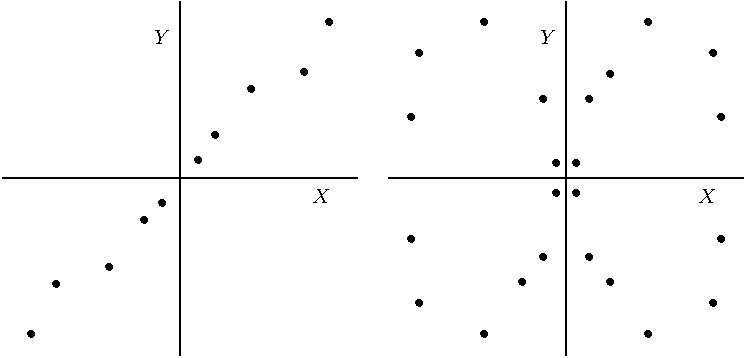
\includegraphics[scale=0.5]{nube}
 \caption{Nube de puntos con relación lineal y sin relación lineal}
\end{figure}
\end{center}
\end{frame}

\begin{frame}
\begin{itemize}
\item La relación lineal no tiene por que ser perfecta. Lo que nos interesa es medir esa
relación lineal.
\item  En el gráfico de la izquierda de la figura~\ref{LINEAL} se vislumbra una
relación lineal mayor que en el de la derecha ya que podemos encontrar un a recta que
aproxime mejor  $Y$ en función de $X$.
\item 
Vamos  a introducir un coeficiente que mide la relación lineal   entre
 dos variables. Este coeficiente es el coeficiente de correlación lineal de Pearson
 $r_{XY}$  y se define de la manera siguiente

$$
r_{XY}=\frac{s_{XY}}{\sqrt{s^2_{X}s^2_{Y}}}=\frac{s_{XY}}{s_{X}s_{Y}}.
$$
\end{itemize}
\end{frame}
%\end{document}
\begin{frame}
\frametitle{Propiedades del coeficiente de correlación lineal}
\begin{enumerate}[1)]
\item $-1\leq r_{XY}\leq 1$
\item $r_{XY}=r_{YX}$
\end{enumerate}
\end{frame}
\begin{frame}
  \frametitle{interpretación del coeficiente de correlación lineal}
Interpretación de $r_{XY}$:
\begin{itemize}
\item[-] $r_{XY}>0$ y a medida que  se aproxima a  $1$,
aumenta la relación lineal positiva entre las dos variables $X$ e $Y$; lo que quiere
decir que si $X$  crece, la variable $Y$ también y si   $X$ decrece,  $Y$  también,
Obsérvese la parte  izquierda de la figura \ref{LINEAL} como ejemplo de este caso.
 \item[-] $r_{XY}<0$  y su valor está muy cerca de -1 quiere
 decir  que hay una buena relación lineal negativa entre las dos variables $X$
 e $Y$; lo
  que significa que si la variable
  $X$    crece, la variable $Y$ decrece o viceversa. Como ejemplo ver
  el gráfico de la derecha de la figura anterior.
\end{itemize}
\end{frame}

\begin{frame}
\begin{figure}
\begin{center}
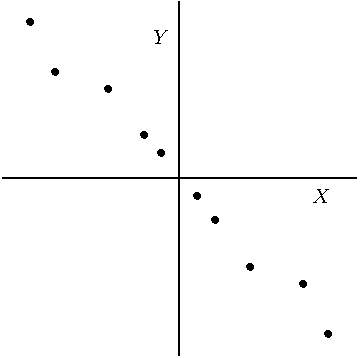
\includegraphics[scale=0.1]{nube2}
\end{center} \caption{Nube de puntos con  relación lineal negativa }
\label{LINEALNEGATIVA}
\end{figure}
\end{frame}

\begin{frame}
\begin{itemize}
\item Si  $r_{XY}=0$ o es pequeño, quiere decir que no hay ningún tipo de relación lineal
  entre las variables $X$ e $Y$.

\item Si $r_{XY}=\pm 1$, hay relación lineal exacta entre $X$ e $Y$, o sea,
 existen dos números reales
$a$ y $b$    tales que $Y=a + b X$.
\end{itemize}
\end{frame}

\begin{frame}
\frametitle{Ejemplo}
Consideremos la siguiente distribución conjunta de la variable $(X,Y)$:
 %(ver ejemplo\ref{bidi})

Los valores de $s^2_X$, $s^2_Y$ y de $s_{XY}$ son:
$$
s^2_X= 63.888,\quad s^2_Y= 47.222,\quad s_{XY}= 22.222
$$

El coeficiente de correlación lineal vale:
$$r_{XY}=\frac{22.222}{\sqrt{63.888 \cdot 47.222}}
=0.405$$
\end{frame}

\subsection{Correlación ordinal}

\begin{frame}
\frametitle{Correlación ordinal}
\begin{itemize}
\item Vamos a estudiar ahora la relación que existe entre dos  ordenaciones dadas por una
muestra de datos bidimensionales.
\item 
Los estadísticos que miden este tipo de relaciones reciben el nombre de coeficiente de
correlación ordinal y  nos darán  medidas de la similitud de las dos ordenaciones a lo
que se suele llamar concordancia.
\item 
Más concretamente, consideremos un conjunto de individuos  y los ordenamos según dos
criterios.
\end{itemize}
\end{frame}

\begin{frame}
\begin{itemize}
\item  Tendremos así dos ordenaciones de los individuos.
\item  Estas ordenaciones las
podemos disponer como si se tratara de una estadística bidimensional, donde la primera
componente de la observación de un individuo correspondería al número de orden del primer
criterio de ordenación y la segunda componente al otro.
\end{itemize}
\end{frame}

\begin{frame}
\frametitle{Ejemplo}
Por ejemplo consideremos  las observaciones en $5$ humanos de su peso $X$ en Kg. y
estatura $Y$ en metros:

\begin{center}
\begin{tabular}{l|r|r|r|r|}
 Individuo $i$ & $(X_i,Y_i)$ & Orden $X$ & Orden $Y$ \\\hline
 Individuo $1$ & $(80,1.75)$ & 3 & 2 \\
 Individuo $2$ & $(75,1.92)$ & 2 & 4 \\
 Individuo $3$ & $(85,1.67)$ & 4 & 1 \\
 Individuo $4$ & $(66,1.80)$ & 1 & 3 \\
 Individuo $5$ & $(90,2.00)$ & 5 & 5\\\hline
\end{tabular}
\end{center}
\end{frame}

\begin{frame}
Si  ordenamos los individuos en orden ascendente (de menor a mayor) según el peso quedan así:

\begin{center}
\begin{tabular}{l|lllll}
Rango Peso   & 1 & 2 & 3 & 4 & 5\\\hline Individuo & $4$&$2$&$1$&$3$&$5$ \end{tabular}
\end{center}
mientras que si los ordenamos en orden ascendente según su altura:
\begin{center}
\begin{tabular}{l|lllll}
Rango  & 1 & 2 & 3 & 4 & 5\\\hline Individuo & $3$&$1$&$4$&$2$&$5$
 \end{tabular}
\end{center}
\end{frame}

\begin{frame}
\begin{itemize}
\item Tenemos así dos ordenaciones de  números ordinales enteros que reciben el nombre de
rangos
\item El cálculo de rangos se complica en el caso de empates, es decir cuando hay valores repetidos en las series de datos. En estos casos se puede romper el empate de varias maneras.
\item En general podemos escribir:
$$
\begin{array}{cc}
\mbox{para } X \rightarrow & \{r_{x_1},r_{x_2}, r_{x_3},\ldots, r_{x_n}\}, \\ 
\mbox{para } Y \rightarrow & \{r_{y_1},r_{y_2}, r_{y_3},\ldots, r_{y_n}\},
\end{array}
$$
\end{itemize}
\end{frame}

\begin{frame}
\begin{itemize}
\item Donde los valores de $r_{x_i}$ y $r_{y_i}$ dan el lugar que ocupa el valor $x_i$ o el
$y_i$ en cada una de las muestras ordenadas.
\item  Estos valores están comprendidos entre $1$ y $n$, luego
son dos permutaciones de orden $n$.
\item Las diferencias entre las ordenaciones son $d_i=r_{x_i}-r_{y_i}\, ; i=1,2,\ldots,n$.
\item El coeficiente de correlación ordinal o por rangos de Spearman queda definido por:
$$
r_S= 1-\frac{6\sum\limits_{i=1}^n d^2_i}{n \left(n^2-1\right)}.
$$
\item 
De hecho, $r_S$ no es más que el coeficiente de correlación lineal introducido en la
sección anterior aplicado a los rangos.
\end{itemize}
\end{frame}

\begin{frame}
\frametitle{Propiedades de $r_S$:}
El coeficiente de correlación lineal  $r_S$ cumple las propiedades siguientes:

\begin{itemize}
\item[-] Si $r_S  = 1$, las dos ordenaciones coinciden; o sea,
$r_{x_i}=r_{y_i}$ para cualquier $i$ entre $1$ y $n$.

\item[-] Si $r_S  = -1$, la ordenación de  $Y$ es exactamente la opuesta a la de $X$, es decir
,  $r_{x_i}=r_{y_{n-i+1}}$  para cualquier $i$ entre $1$ y $n$.

\item[-]  El coeficiente $r_S$ esta siempre comprendido  entre -1
y 1. Si $r_S  >0$, podemos decir   que las dos ordenaciones son del mismo sentido
 y si $r_S <0$, las dos ordenaciones son de sentidos opuestos.
\end{itemize}
\end{frame}

\begin{frame}
\frametitle{Ejemplo}

Consideremos la muestra anterior de pesos y estaturas de $5$ individuos:

\begin{center}
\begin{tabular}{l|r|r|r|r|}
 Individuo $i$ & $(X_i,Y_i)$ &  $r_{X_i}$ &$r_{Y_i}$ & $d^2_i$ \\\hline
 Individuo $1$ & $(80,1.75)$ & $3$ & $2$ & $1$\\
 Individuo $2$ & $(75,1.92)$ & $2$ & $4$ & $4$\\
 Individuo $3$ & $(85,1.67)$ & $4$ & $1$ & $9$\\
 Individuo $4$ & $(66,1.80)$ & $1$ & $3$ & $4$\\
 Individuo $5$ & $(90,2.00)$ & $5$ & $5$ & $0$\\\hline
 $\Sigma$ & & & & $18$
\end{tabular}
\end{center}
\end{frame}

\begin{frame}
Luego tenemos que :

$$
r_s = 1 -  \frac{6\cdot 18}{5\cdot (25-1)}= 1-\frac{108}{120}= 0.1
$$

\end{frame}






\section{Apéndice estadística descriptiva}
%%%%%%&AL APENDICE SI HAY
\subsection{Medias armónica y geométrica}
\begin{frame}
\frametitle{Medias armónica y geométrica}
\begin{itemize}
\item Las medias armónica y geométrica no son de gran utilidad salvo en problemas concretos. Se
calculan de la siguiente forma:
\item Media Armónica: $M_{h}=\frac{n}{\sum\limits_{i=1}^{n} \frac{1}{x_i}}=\frac{n}{\sum\limits_{j=1}^{I} \frac{n_j}{X_j}}$.
\item Media geométrica: $M_g=\root n\of{\prod_{i=1}^{n} x_j} =\root n\of{\prod_{j=1}^{I} X_j^{n_j}}$.
\item Estas medias tienen restricciones sobre los datos, no pueden tener datos nulos, y en
general se utilizan para datos positivos.
\end{itemize}
\end{frame}


\subsection{Media general de orden m}

\begin{frame}
\frametitle{Media general de orden $n$}
\begin{itemize}
\item Definimos la media general $M_{(m)}$ de orden $m$ como 
$M_{(m) }=\left(\frac{\sum_{i=1}^n  n_i x_i^m}{n}\right)^{\frac{1}{m}}=
\left(\frac{\sum_{j=1}^J  n_j X_j^m}{n}\right)^{\frac{1}{m}}$.
\item Se cumple que $M_{(-1)}=M_h;\,  M_{(0)}=M_g;\,  M_{(1)}=\overline{x}$.
\item Además se cumple que $M_{(m)}$ es una función creciente en $m$ y por lo tanto :
$M_h\leq M_g\leq \overline{x}.$
\end{itemize}
\end{frame}

\subsection{Moda para datos agrupados}

\begin{frame}
\frametitle{Moda}
\begin{itemize}
\item Hay algunos algoritmos para aproximar la moda  para datos agrupados.
\item Si los intervalos tienen la misma amplitud, podemos aproximar la moda de la siguiente manera-
\item En primer lugar localizamos el intervalo con frecuencia absoluta más alta.
\item Sean $[L_c, L_{c+1})$ los extremos del intervalo con  frecuencia absoluta máxima.
\end{itemize}
\end{frame}

\begin{frame}
\begin{itemize}
\item Para calcular la moda podemos utilizar  la siguiente  fórmula, en la que suponemos que
todos los intervalos tienen la misma amplitud $A$ (en caso contrario se utilizan otras
aproximaciones):

$$M_o =L_c + A \frac{n_{c+1}}{(n_{c-1}+n_{c+1})}.$$

\item Donde:
\begin{itemize}
\item $A$: amplitud de los intervalos
\item $n_{c-1}$: frecuencia absoluta del intervalo anterior al de
frecuencia máxima.
\item $n_{c+1}$: frecuencia absoluta del intervalo posterior al de
frecuencia máxima.
\end{itemize}
\end{itemize}
\end{frame}

\begin{frame}
\frametitle{Ejemplo}
Consideremos la siguiente distribución de frecuencias: 
\begin{center}
\begin{tabular}{lccc}
intervalos    & $X_j$ & $n_j$ & $N_j$ \\ \hline $[1.5,4.5) $  &  \ 3 & \ 3 &   \ 3  \\
$[4.5,7.5) $  &  \ 6 &  12 &  15  \\ $[7.5,10.5)$  &  \ 9 &   \ 5 &  20
\\ $[10.5,13.5)$ & 12 &   \ 4 &  24  \\ \hline
\end{tabular}
\end{center}
\end{frame}
\begin{frame}
El intervalo con la frecuencia absoluta mas alta es el $[4.5,7.5)$. Por lo tanto, la moda
vale:

$$M_0=4.5+3\frac{5}{(3+5)}=6.375.$$
\end{frame}


\subsection{Desviación media}

\begin{frame}
\frametitle{Desviación media}
\begin{itemize}
\item La desviación media es un índice de dispersión respecto a la mediana o a la media. Queda
definido por: $D_M=\frac{1}{n}\sum\limits_{j=1}^{J}n_j|X_j - M|.$
\item Donde $M$ es la mediana o la media aritmética.
\item La propiedad fundamental de la desviación  media respecto a la mediana es que minimiza
las desviaciones en valor absoluto respecto de un punto cualquiera $X_0$. Es decir $\mbox{mín}_{X_0} \frac{1}{n} \sum\limits_{j=1}^{J}n_j|X_j - X_0|=D_M.$
\end{itemize}
\end{frame}

\subsection{Recorrido}
\begin{frame}
\begin{itemize}
\item Otra medida de dispersión es el recorrido. Se define como la diferencia entre el valor
máximo y mínimo de los valores observados.
\item Consideremos la siguiente distribución de frecuencias:
\begin{center}
\begin{tabular}{lrrr}
intervalos &\multicolumn{1}{c}{$X_j$} & \multicolumn{1}{c}{$n_j$}
&\multicolumn{1}{c}{$n_j X_j$}\\ \hline $[0.5,15.5) $ &  8 & 4  & 32  \\ $[15.5,30.5)$ &
23 & 4 & 92 \\ $[30.5,45.5)$ & 38 & 2 & 76 \\
 \hline
Sumas     &      & 10 & 200
\end{tabular}
\end{center}
\item  Vamos a calcular la desviación media:
\end{itemize}
\end{frame}

\begin{frame}
\begin{itemize}
\item Calculamos la media $\overline{x}=\frac{200}{10}=20$.
\item Añadimos dos columnas más a la tabla de frecuencias:
\begin{center}
\begin{tabular}{ccc}
$X_j$  & $|X_j-\overline{x}|$ &  $n_j|X_j-\overline{x}|$ \\ \hline \ 8     & 12   &   48
\\ 23     & \ 3     &  12  \\ 38     & 18     &  36   \\ \hline Sumas  &       &  96 \\
\end{tabular}
\end{center}
\item  La desviación media es $D_M=\frac{96}{10}=9.6$.
\end{itemize}
\end{frame}

\begin{frame}
También se utiliza el recorrido intercuartílico que es $Q_{0.75}-Q_{0.25}$; la diferencia entre el
tercer y primer cuartil. También se pueden calcular recorridos con deciles, percentiles y
cuantiles en general.
\end{frame}
